\chapter{Extensão das funcionalidades}

No capítulo anterior, foi apresentada uma visão geral do sistema e alguns de seus principais componentes. Esse capítulo tem como objetivo descrever as implementações da extensão realizada.

As extensões foram realizadas em diferentes componentes da base. Novas tabelas foram adicionadas ao banco de dados para apresentação dos dados em tempo real. Uma nova interface foi acoplada ao servidor e o novo modelo de propagação foi implementado, visando aumentar a acurácia da resposta do servidor referente à quantidade de canais livres no espectro de frequência.

\section{\textit{Frontend} }

O termo \textit{frontend} se refere à camada de apresentação dos dados e interação com o usuário final. No trabalho atual, visando facilitar a interação do usuário com o servidor e exibir as informações presentes na resposta das requisições em um formato mais apresentável, foi implementada uma página Web responsiva, na qual o usuário é capaz, através de um mapa, de consultar a base e obter a quantidade de canais livres. Também é apresentado um mapa de calor representando a distribuição de canais livres em uma porção região sudeste do Brasil.
Para o desenvolvimento da página Web, foi necessário o uso de um conjuno de tecnologias, apresentadas a seguir.

\
\subsection{HTML}

Considerada a linguagem de marcação da World Wide Web ~\cite{htmlw3cs}, o \textit{HyperText Markup Language} (HTML) é a base do \textit{frontend}, servindo como o esqueleto da página. Todas as outras tecnologias implementadas trabalham sobre os elementos inicialmente criados nessa linguagem.

Foi criada pelo físico britânico Tim Berners-Lee, também criador do HTTP,
na década de 90. Inicialmente, Tim tinha a intenção de resolver um problema no laboratório onde trabalhava, o European Organization for Nuclear Research, também chamado de CERN. Diversos artigos científicos citavam outros, que por sua vez citavam outros artigos relacionados. Essa distribuição de conhecimento dificultava o acesso rápido e prático às informações, pois era necessário saber em qual máquina estava armazenado fisicamente determinado artigo para acessá-lo, acessá-la e salvar o arquivo em uma unidade de armazenamento externa.

Com isso, Tim buscou criar documentos estruturados, baseados em \textit{
tags}, que estariam interconectados. Com isso, bastaria um click para acessar um documento relacionado, formando uma rede de documentos. Surge então, o primeiro protótipo da Web.

Atualmente, o HTML é mantido pela World Wide Web Consortium (W3C) \abbrev{W3C}{World Wide Web Consortion}. Após um longo período sem a publicação de novas versões, sua última versão, visando acompanhar o desenvolvimento da Web nas últimas duas décadas,foi lançado em 2008, o HTML5~\cite{htmlw3cs}.  

Um documento HTML é estruturado por \textit{tags}, de diferentes tipos, para determinar que os dados que estão entre essas \textit{tags} são texto puro, imagem, arquivo de áudio, entre outros formatos possíveis.


\subsection{JavaScript}

Javascript é uma linguagem de programação dinâmica, amplamente utilizada em conjunto com o documento HTML. Ela é utilizada para dinamizar o funcionamento da página Web, através de scripts que podem ser escritos diretamente no arquivo HTML (Através da \textit{tag}), ou em arquivos externos, que são importados pelo HTML.

Atualmente, a linguagem é utilizada não só para melhorar a experiência do usuário nas páginas Web, mas como linguagem de programação dos servidores, com o surgimento de tecnologias como Node.js.

\subsection{CSS}

Com o desenvolvimento da Web, notou-se que as \textit{tags} do HTML estavam ficando muito grandes, com muitos atributos, o que acabava dificultando a manutenção do código. Com isso, visando extrair do HTML os parâmetros referentes ao estilo da página, surgiu o Cascading Style Sheets (CSS) ~\abbrev{CSS}{Cascading Style Sheets}, linguagem utilizada na formatação do estilo da página. Atualmente, sua versão é o CSS3, com suporte à animação de elementos do HTML.

\subsection{Implementação}

Com a utilzação das linguagens citadas anteriormente, foi criada uma página Web, onde o usuário é capaz de observar um mapa de calor representando a ocupação das faixas de frequência no intervalo da Tv analógica, e consultar a base para obter em um ponto específico, a quantidade de canais livres e as informações de frequência dos mesmos.

\subsubsection{Alterações no Servidor}

Para a implementação do Longley-Rice, foram necessárias diversas alterações no servidor previamente desenvolvido. 

Para a criação de um novo objeto modelo, foi necessária a criação de uma classe que herdasse de \textit{PropagationModel}, classe utilizada pelos outros modelos implementados anteriormente. A nova classe \textit{LongleyRice} implementa os métodos \textit{
interferes()} e \textit{maxDistance()}. O método \textit{maxDistance()} determina o alcance máximo do dispositivo, enquanto o método \textit{interferes()} determina se a soma dos raios dos alcances dos dispositivos primário e secundários supera a distância física entre eles.

\begin{lstlisting}

public double maxDistance(TransmissionDevice dev, TransmissionDevice ant)

\end{lstlisting}

\subsubsection{Estrutura da Página}

Ao carregar a página, o mapa é apresentado na direita, e quatro opções na esquerda. Essas opções consistem no modelo a ser exibido. Dentro do mapa, há um marcador que pode ser movido e em seguida uma consulta é enviada ao servidor, passando como parâmetro a localização do marcador e o modelo selecionado, em seguida uma lista é apresentada, com os canais livres e sua frequência.

%O sistema foi desenvolvido na linguagem de programação orientada a objeto Java, usando o Sistema de Gerenciamento de Banco de Dados (SGBD)
%\abbrev{SGBD}{ Sistema de Gerenciamento de Banco de Dados}
%MYSQL como banco de dados. A API foi desenvolvida no protocolo REST, utilizando a biblioteca restlet~\cite{restlet}, e utilizando XML como formato de resposta. O desenvolvimento foi feito no ambiente Eclipse~\cite{eclipse}, e os diagramas de classe aqui exibidos foram gerados utilizando o plug-in ObjectAid.
%
%A escolha pela linguagem de desenvolvimento Java ocorreu devido a maior familiaridade com a linguagem e as capacidades multiplataforma dela. O sistema foi desenvolvido no sistema operacional Windows 7, mas foi devidamente testado em um ambiente Linux utilizando uma máquina virtual. A ferramenta de virtualização utilizada foi a Oracle VM BOX~\cite{vmbox}.
%
%Pode-se descrever o programa desenvolvido como sendo a etapa de pedido de disponibilidade do PAWS. Pode-se descrever o funcionamento em linhas gerais em quatro módulos. Como indicado na figura~\ref{fig:SAM}.
%
%\begin{figure}[htb]
%\centering
%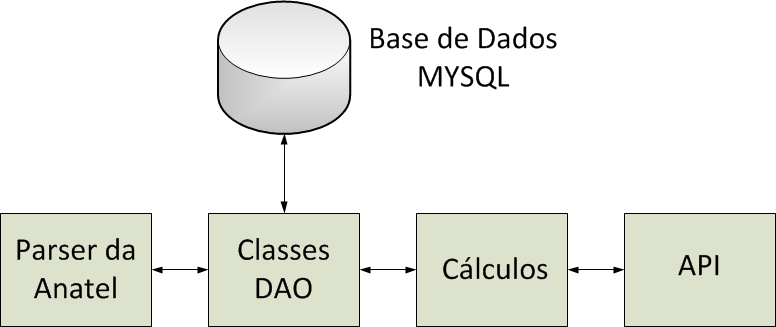
\includegraphics[width=0.8\textwidth]{figs/sam}
%\caption[\textit{Diagrama do Sistema Desenvolvido}.]
%{Diagrama geral do sistema desenvolvido.}
%\label{fig:SAM}
%\end{figure} 
%
%
%Cada um desses módulos será descrito no decorrer do capítulo.
%
%
%\subsection{Desenvolvimento}
%
%Deve ser ressaltado que o objetivo do trabalho foi desenvolver um sistema que ofereça a funcionalidade básica de prover os canais disponíveis do WS mas que seja facilmente modificado para a adição de outras funções. Para facilitar o reuso do trabalho foi adotado o padrão de desenvolvimento de Fábrica~\cite{cooper2000java}. Resumidamente, as interfaces que cada objeto deve estender são definidas, e existem objetos fábricas, responsáveis por criar instâncias de objetos que estendam essa interface. Dessa maneira, nenhum objeto é referenciado diretamente.
%
%
% Tome como exemplo as classes onde foram implementados os modelos de propagação. Existe a interface \textit{PropagationModel}, que define as características básicas de um modelo de propagação. Ela possui o método abstrato \textit{maxDistance} que serve para determinar o alcance máximo de cada dispositivo de transmissão. Cada classe que implemente um modelo de propagação estende essa interface  e implementa esse método. Durante o programa quando é necessário utilizar algum modelo de propagação nunca é criado um objeto diretamente das classes, mas é invocada a classe\textit{PropagationModelFactory} que retorna um objeto que estenda a interface \textit{PropagationModel}.
%
%Um diagrama com as classes factories está na figura~\ref{fig:facto}.
%
%\begin{figure}[htb]
%\centering
%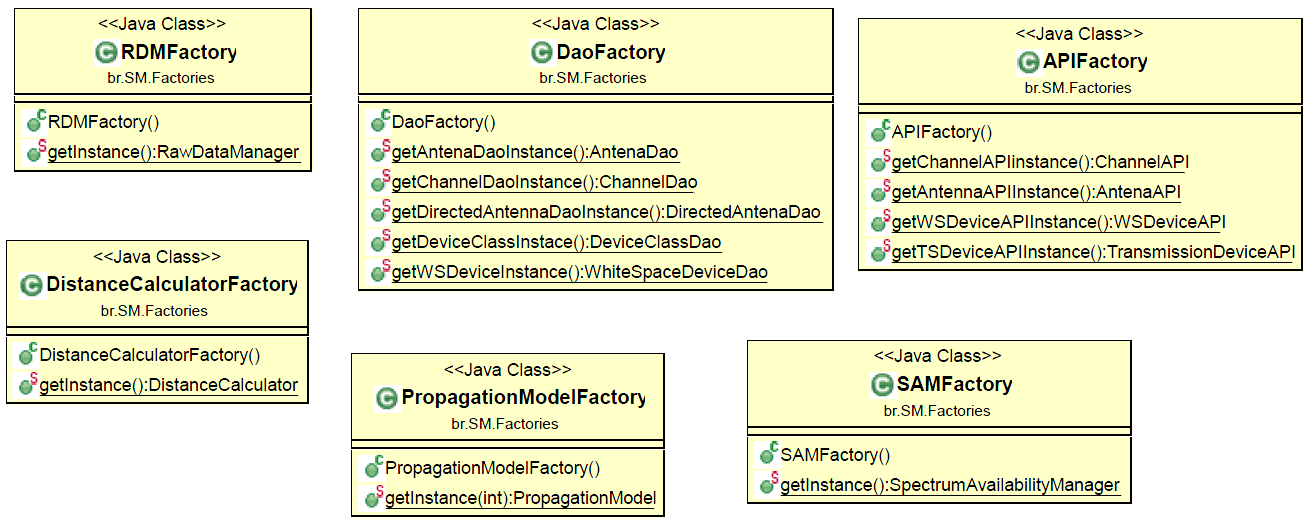
\includegraphics[width=1.0\textwidth]{figs/factories}
%\caption[\textit{Factories}.]
%{Diagrama de classe das - \textit{Factories} }
%\label{fig:facto}
%\end{figure} 
%
%
%Dessa maneira o conteúdo das classes é abstraído. Um desenvolvedor deve apenas se preocupar em obedecer as interfaces. A interface define o modo como possíveis classes serão utilizadas, definindo todos os métodos acessáveis por outros objetos.
%
%
%\subsection{Definições}
%
%Para calcular a disponibilidade de canais no WS foi utilizada uma aproximação bem direta. 
%
%Com as informações sobre as antenas existentes no Estado do Rio de Janeiro é possível calcular o alcance máximo de cada antena. Por alcance máximo se entende: ``A distância máxima da base da antena que um dispositivo pode estar para receber o sinal transmitido por ela com uma relação sinal/ruído mínima. Assume-se que o dispositivo não sofre nenhuma interferência além de duas vezes ruído de fundo''. Todos os dispositivos dentro do alcance da antena vão receber o sinal com qualidade suficiente. Para dispositivos fora desse alcance, a qualidade do sinal recebido será muito baixa, de modo que USs não estariam em condição de interferência com a antena.
%
%Assumindo um US pode-se calcular seu alcance de forma similar ao da antena. A diferença é que o alcance de um US é igual à distância necessária para que sua potência seja atenuada até o valor do ruído de fundo.
%
%A interferência nos receptores de A de duas vezes o ruído de fundo é devido ao ruído normal do ambiente somado à potência do sinal irradiado por um US que já sofreu atenuação.
%
%Assumindo uma antena A com alcance \begin{math}d_1\end{math} e um US B com alcance \begin{math}d_2\end{math}. Sendo D a distância entre A e B. Define-se que o dispositivo B interfere os receptores da antena A se e somente se:
%
%\begin{align}
%  \label{interfere} d_1 + d_2 \leq D
%\end{align}
%
%
%Um exemplo de interferência está na figura~\ref{fig:interf}.
%
%\begin{figure}[htb]
%\centering
%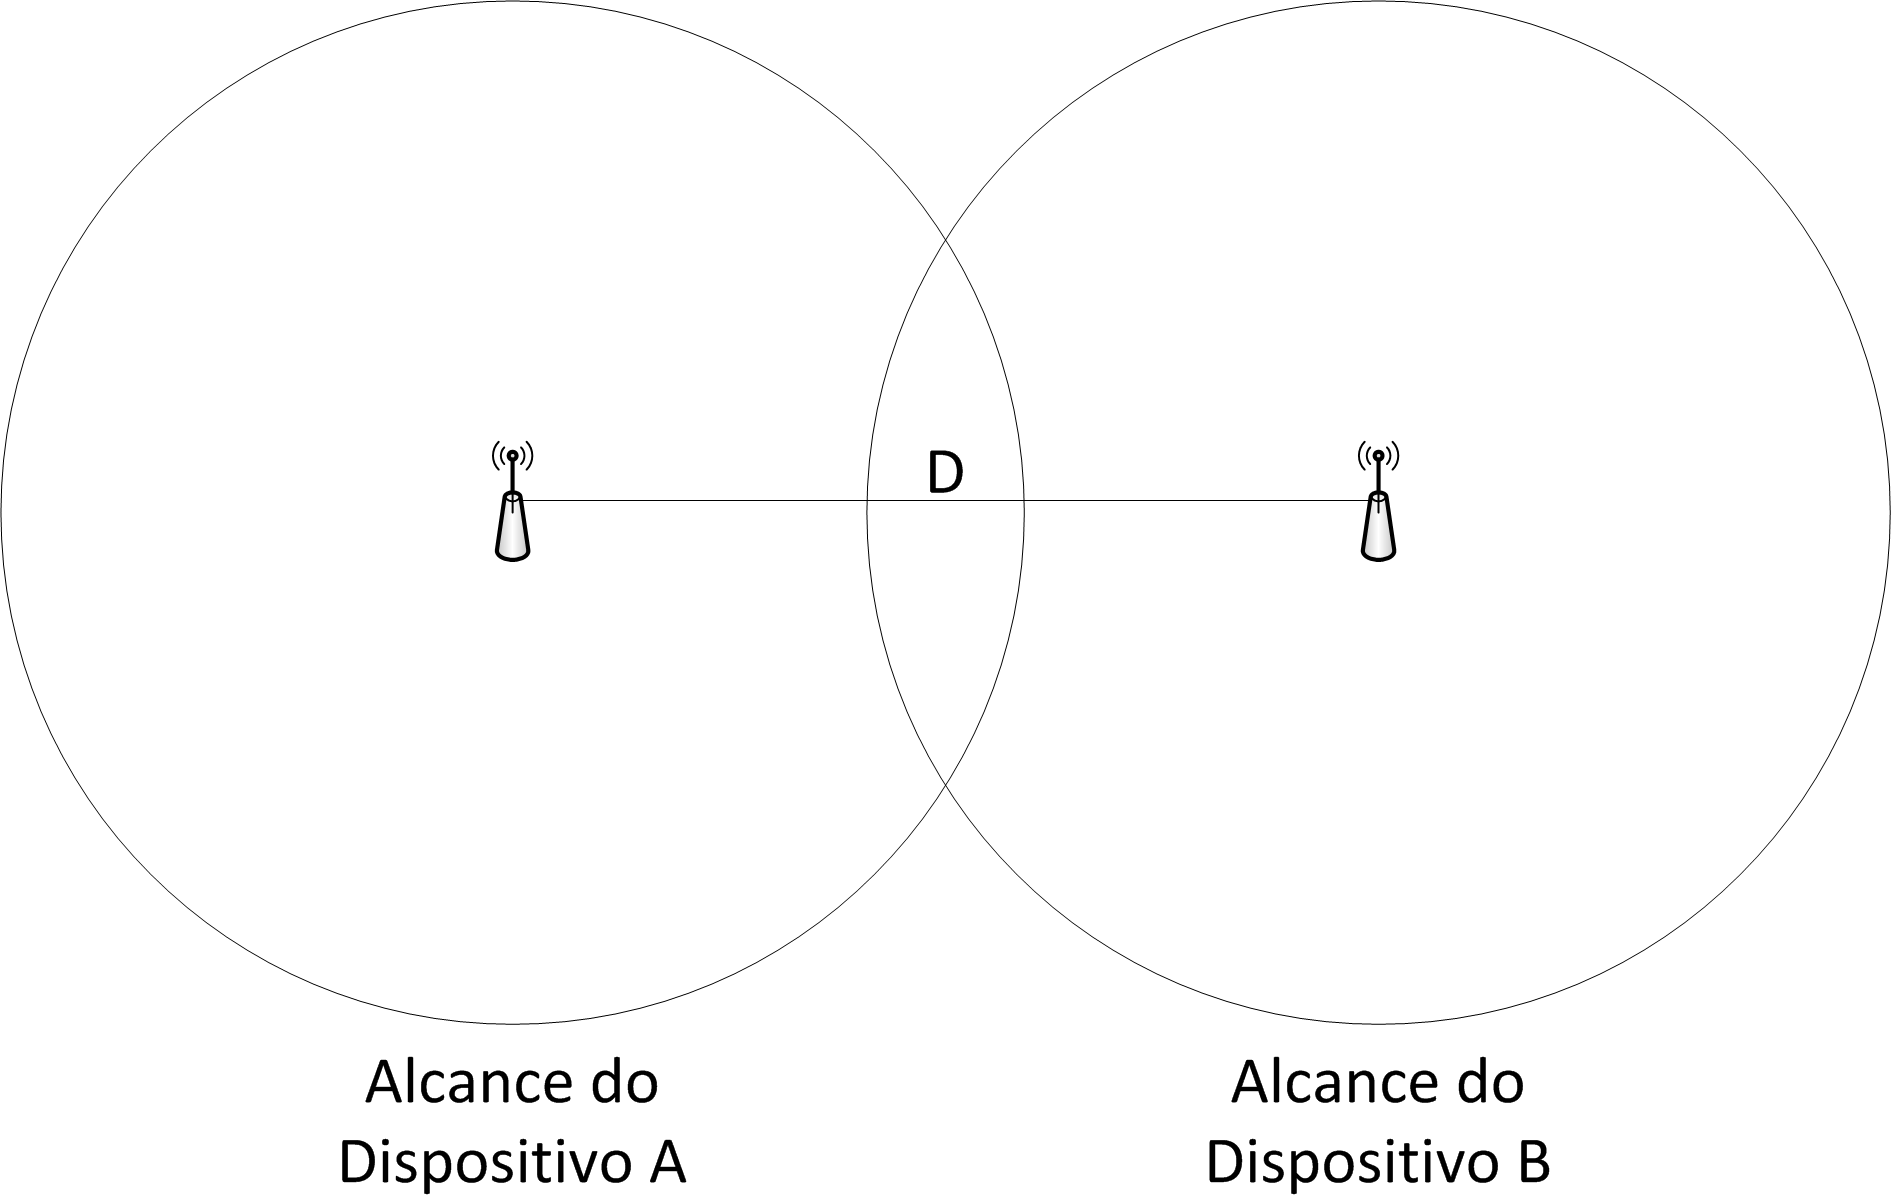
\includegraphics[width=0.8\textwidth]{figs/Interf}
%\caption[\textit{Interferência}.]
%{Exemplo de Interferência.}
%\label{fig:interf}
%\end{figure} 
%
%Se o dispositivo B interferir nos receptores da antena A, o canal que A utiliza para transmissão se torna indisponível para B. Os canais que não possuam antenas em interferência com o dispositivo B estão disponíveis para uso.
%
%O valor de D é calculado pela distância entre a antena e o dispositivo no globo terrestre. Já o cálculo de \begin{math}d_1\end{math} e \begin{math}d_2\end{math} será explicado na seção ``Determinação do White Space''
%
%
%\section{Coleta de dados}
%
%Antes de entrar em operação, o sistema deve construir sua base de dados com as informações necessárias para os cálculos. Como foi indicado, é importante a existência de informações sobre todas as antenas do Rio de Janeiro. A falta de informação culmina na inviabilidade do projeto.
%
%A informações foram acessadas no site da ANATEL~\cite{siscom}. Os dados foram obtidos de forma manual, não existe um Web Service, ou alguma forma de comunicação direta com a agência reguladora brasileira.
%
%Foi baixado um arquivo com informações sobre todas as antenas de televisão do Brasil. Esse arquivo está no formato TSV (Tab Separated Values) onde cada linha contém as informações de uma antena conforme abaixo:
%
%\begin{itemize}
%\item Estado
%\item Cidade
%\item Dono
%\item Tipo
%\item Canal
%\item Complemento do Canal 
%\item Campo Vazio
%\item Latitude 
%\item Longitude 
%\item Potência
%\item Informações de Antenas Direcionais
%\end{itemize}
%
%Foram utilizadas apenas as linhas onde o campo \textit{Estado} era "RJ". 
%
%O campo \textit{Canal} e \textit{Complemento do Canal} foram utilizados para identificar o canal onde determinada antena opera.
%
%Os campos \textit{Latitude} e \textit{Longitude} estão no formato grau-minuto-segundo, com uma letra indicando a direção da bússola. Esses valores foram convertidos para o formato decimal, que é considerado um formato mais padronizado, e por facilitar as contas que serão feitas. Esses campos identificam a posição da antena no planeta Terra.
%
%O campo \textit{Potência} está em kW, sendo utilizado para determinar a potência de transmissão da antena.
%
%Para esse trabalho as antenas foram consideradas como sendo multidirecionais, ou seja, irradiam com a mesma potência em todas as direções. No entanto, existem antenas direcionais, que irradiam com uma determinada potência apenas em um cone direcionado. As informações específicas dessas antenas direcionais estão nos campos \textit{Informações de Antenas Direcionais}. Essas informações constituem de um trio de campos para cada antena direcionada existente nessa posição. Todas as antenas direcionadas estão operando no mesmo canal, apenas com potências e direcionamentos diferentes.
%
%As seguintes informações são indicadas para antenas direcionadas:
%
%\begin{itemize}
%\item Altura
%\item Direcionamento (Azimuth)
%\item Potência
%\end{itemize}
%
%Esses três campos também são utilizados pelo sistema.
%
%
%\subsection{Implementação}
%
%Existe um parser responsável por converter o arquivo extraído da ANATEL em uma lista de objetos \textit{Antena}. As informações sobre antenas direcionadas são incluídas em uma lista de objetos  \textit{DirectedAntena}, que é associada a \textit{Antena} que ela pertence.
%
%O diagrama na figura~\ref{fig:antena} especifica esse exemplo.
%
%\begin{figure}[htb]
%\centering
%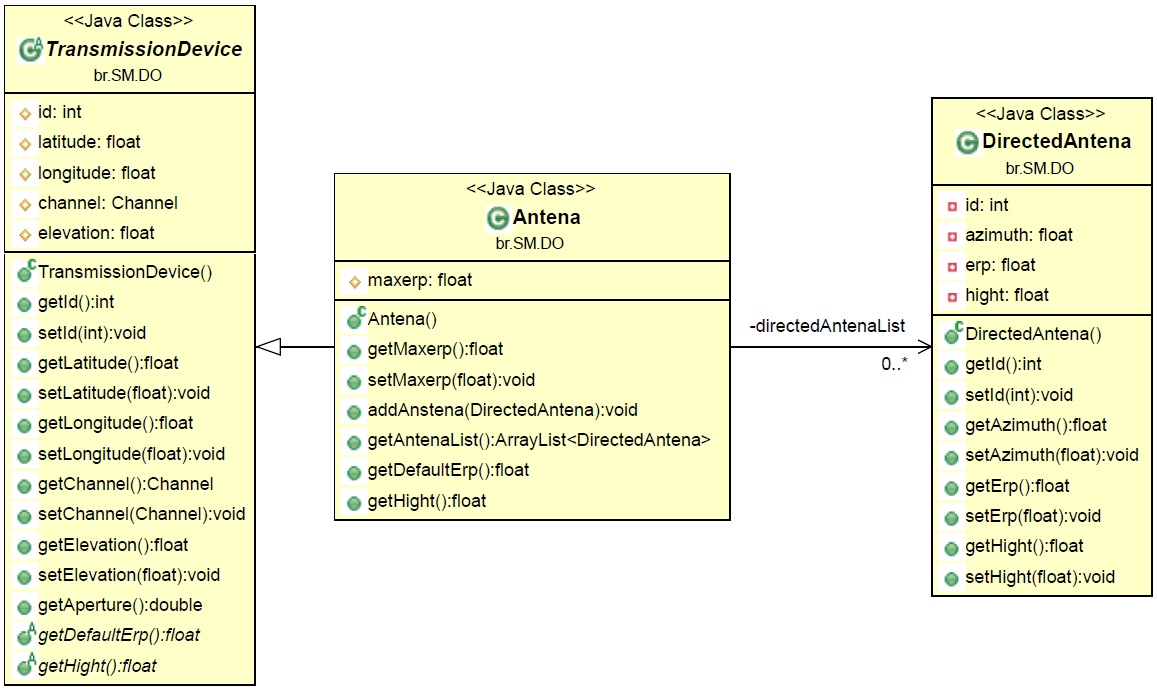
\includegraphics[width=1.0\textwidth]{figs/antena}
%\caption[\textit{Antena}.]
%{Diagrama de classes das antenas.}
%\label{fig:antena}
%\end{figure} 
%
%O parser pode, também, buscar a altura geográfica de onde as antenas se encontram. Isso é feito usando Google Elevation API~\cite{elevation}. Essa informação só é utilizada pelo sistema caso não exista nenhuma informação sobre altura no arquivo da ANATEL.
%
%O diagrama de classes para esse módulo está na figura~\ref{fig:RDM}.
%
%\begin{figure}[htb]
%\centering
%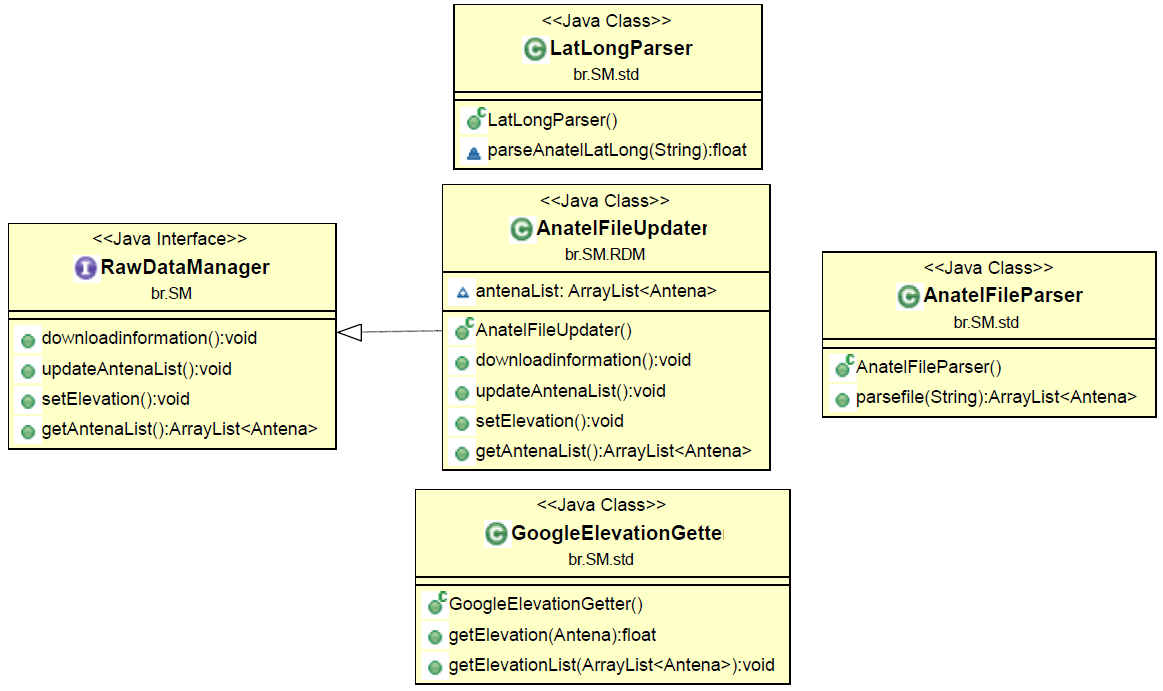
\includegraphics[width=1.0\textwidth]{figs/rdm}
%\caption[\textit{Parser}.]
%{Diagrama de classes do módulo\textit{Parser}.}
%\label{fig:RDM}
%\end{figure}
%
%
%
%\subsection{Extensão}
%
%A obtenção de dados é abstraído para a interface \textit{RawDataManager}. Assim sendo, caso seja determinada uma nova maneira para comunicação com a ANATEL, basta que um método herde a interface antes mencionada. 
%
%Na figura~\ref{fig:parse} está indicado como ocorre o parsing do arquivo da ANATEL sob um ponto de vista de classes utilizadas.
%
%\begin{figure}[htb]
%\centering
%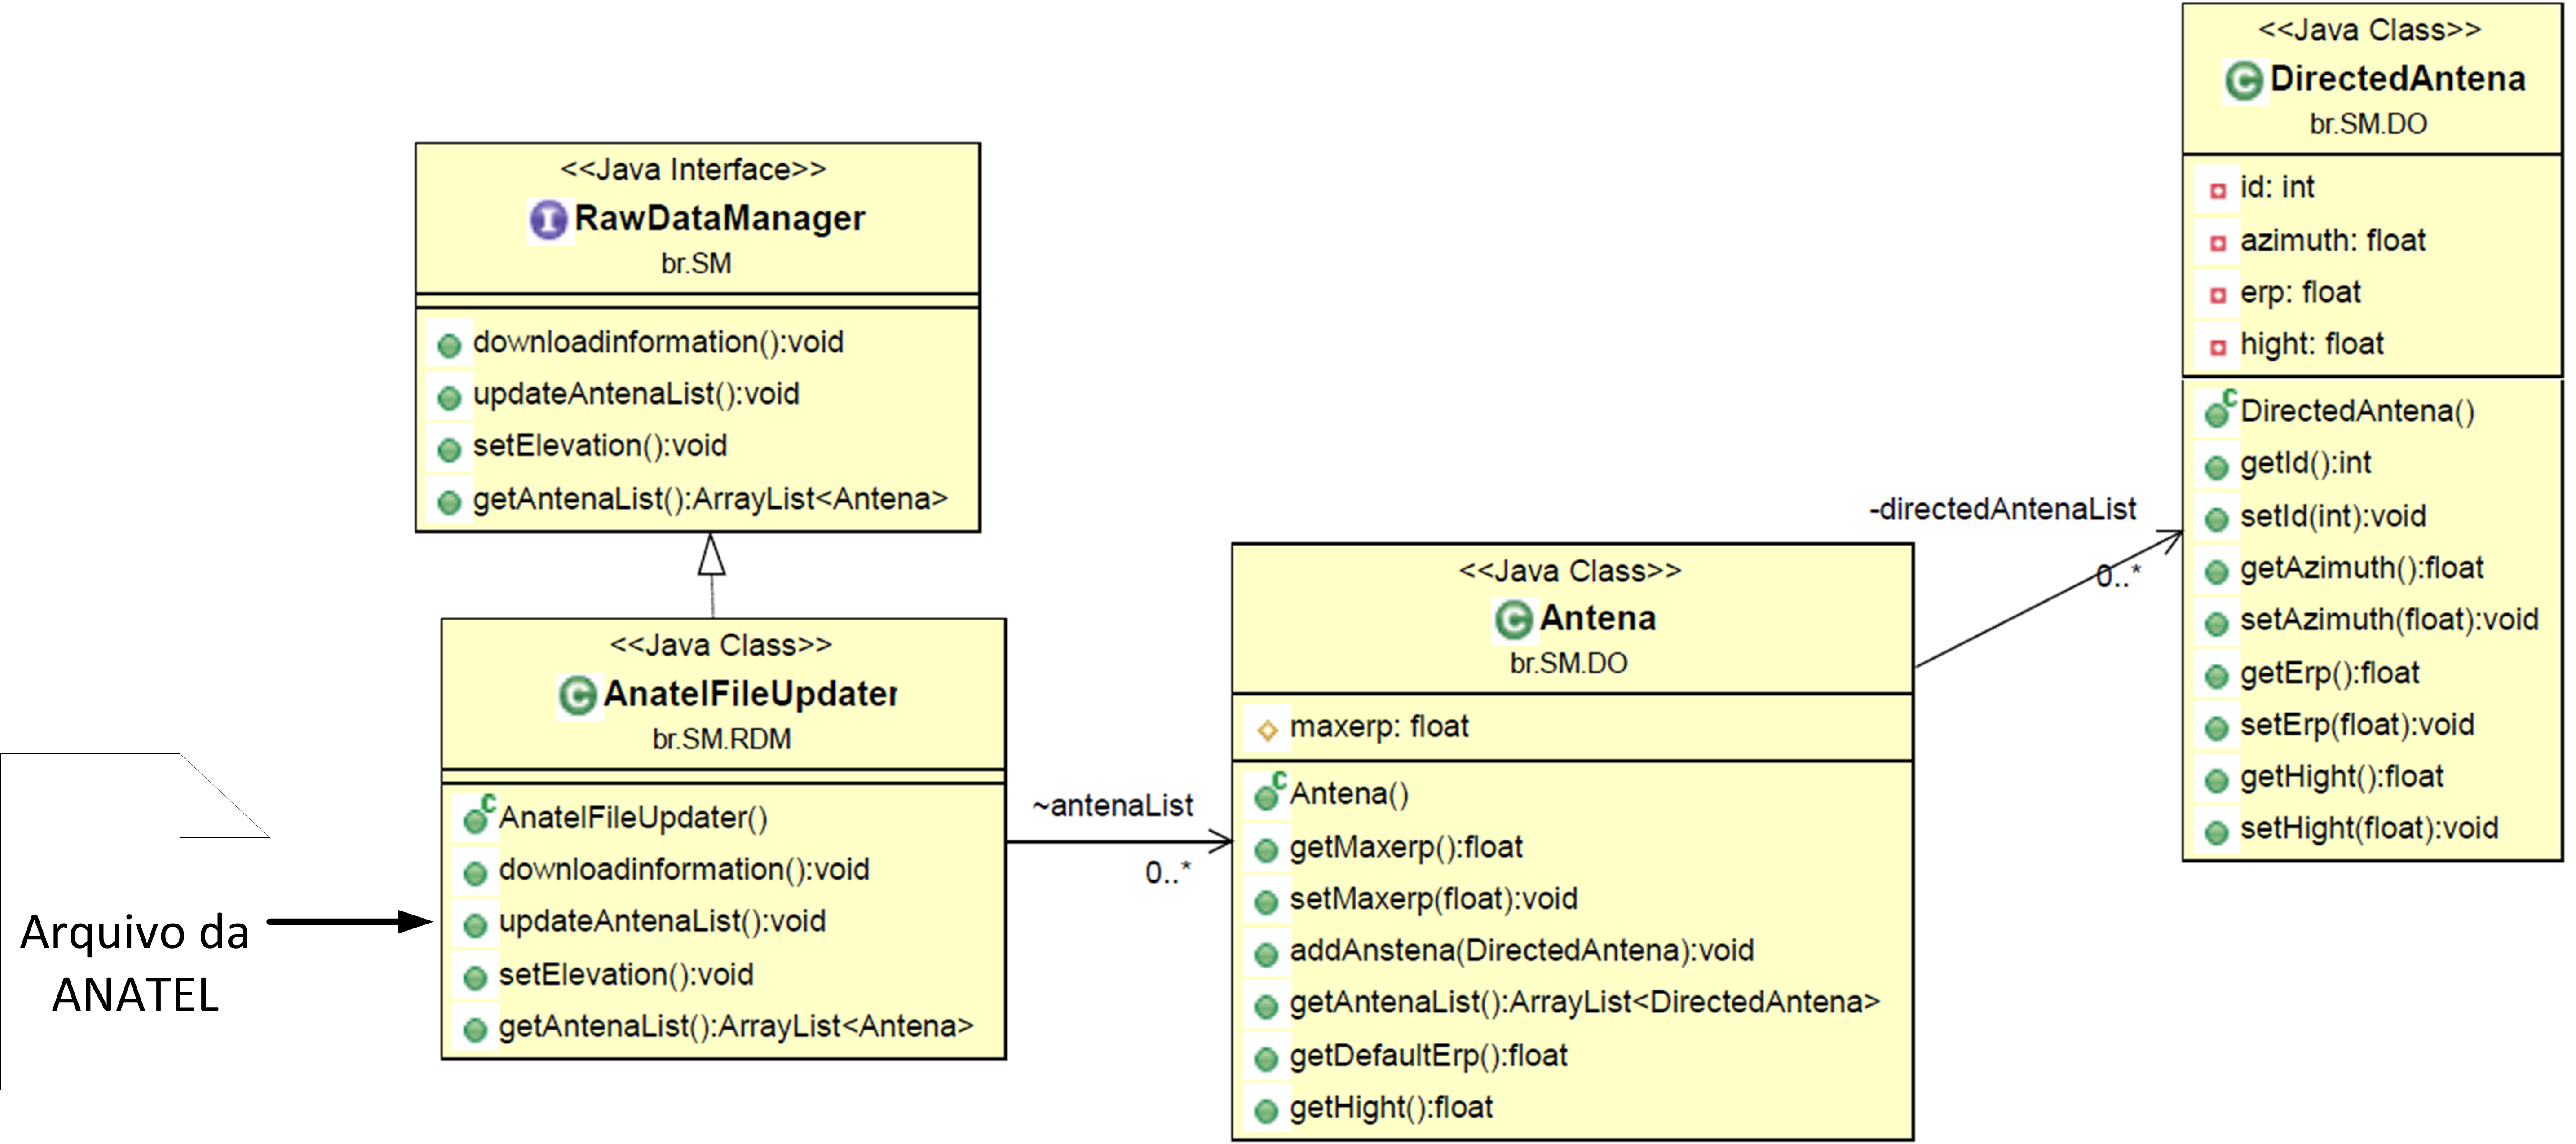
\includegraphics[width=1\textwidth]{figs/rdmext}
%\caption[Diagrama com o processo de Parsing.]
%{Diagrama com o processo de Parsing.}
%\label{fig:parse}
%\end{figure}
%
%
%\subsection{Qualidade da Informação}
%
%
%Como já foi indicado, garantir a qualidade da informação que é obtida da ANATEL é essencial para a BDWS criada. No entanto, foram encontradas algumas informações erradas no arquivo utilizado como fonte.
%
%Para testar a qualidade da informação utilizada foi gerado um arquivo KML~\cite{KML} com a localização das antenas. Foi utilizado o Google Earth para verificar visualmente a posição das antenas~\cite{gearth}.
%
%\begin{figure}[htb]
%\centering
%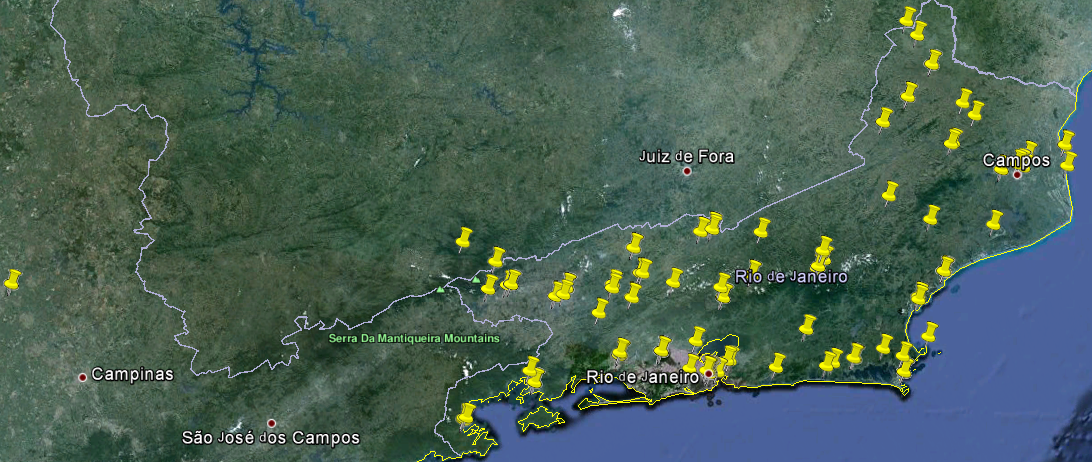
\includegraphics[width=1.0\textwidth]{figs/antenamap}
%\caption[Vizualização de antenas indicadas pela ANATEL.]
%{Vizualização de antenas indicadas pela ANATEL.}
%\label{fig:antenamap}
%\end{figure} 
%
%Como se pode ver na figura~\ref{fig:antenamap}, algumas das antenas que estavam indicadas como localizadas no Rio de Janeiro pertenciam, na verdade, a São Paulo.
%
%Outro ponto identificado são valores, a princípio, estranhos. Alguns valores de potência estão muito maiores que o esperado para uma antena.
%
%É preciso firmar com a ANATEL uma relação de cooperação para aprimorar a base. Isso será discutido mais a fundo no capítulo 6 na seção de trabalhos futuros.
%
%Vale ressaltar que o formato adotado pela ANATEL para armazenar latitude e longitude é muito impreciso. A agência só armazena o grau, minuto e segundo de cada coordenada geográfica, faltando informações sobre décimos e centésimos de segundo. Essa falta de precisão na localização das antenas deve ser corrigida a fim de prover informações o mais corretas possível.
%
%\section{Base de Dados}
%
%
%Além das informações obtidas da ANATEL a base de dados armazena, também, informações sobre reservas de canais feitas pelos DSs. Na modelagem de dados feita foi criada a classe \textit{TransmissionDevice}, da qual foram estendidas as classes \textit{Antena} e \textit{WhiteSpaceDevice}. A diferença básica entre esses dois objetos é que a \textit{Antena} possui uma potência de transmissão informada pela ANATEL e uma lista de \textit{DirectedAntena} a qual está associada. Já o \textit{WhiteSpaceDevice} está associado a uma classe de dispositivo (\textit{DeviceClass}) que tem uma potência predeterminada.
%
%Foram criadas três classes de dispositivos:
%
%\begin{itemize}
%\item "INTERNO BAIXO" com potência de 10 miliwatts
%\item "INTERNO ALTO" com potência de 50 miliwatts
%\item "EXTERNO" com potência de 100 miliwatts
%\end{itemize}
%
%As classes do tipo ``INTERNO'' representam dispositivos para uso interno, ou seja, dentro de alguma construção. Já a classe do tipo ``EXTERNO'' representa dispositivos para uso externo.
%
%Classes criadas para representar antenas e DS, também chamadas de classes de dados, ou Data Objects estão representadas na figura~\ref{fig:DO}.
%
%\begin{figure}[htb]
%\centering
%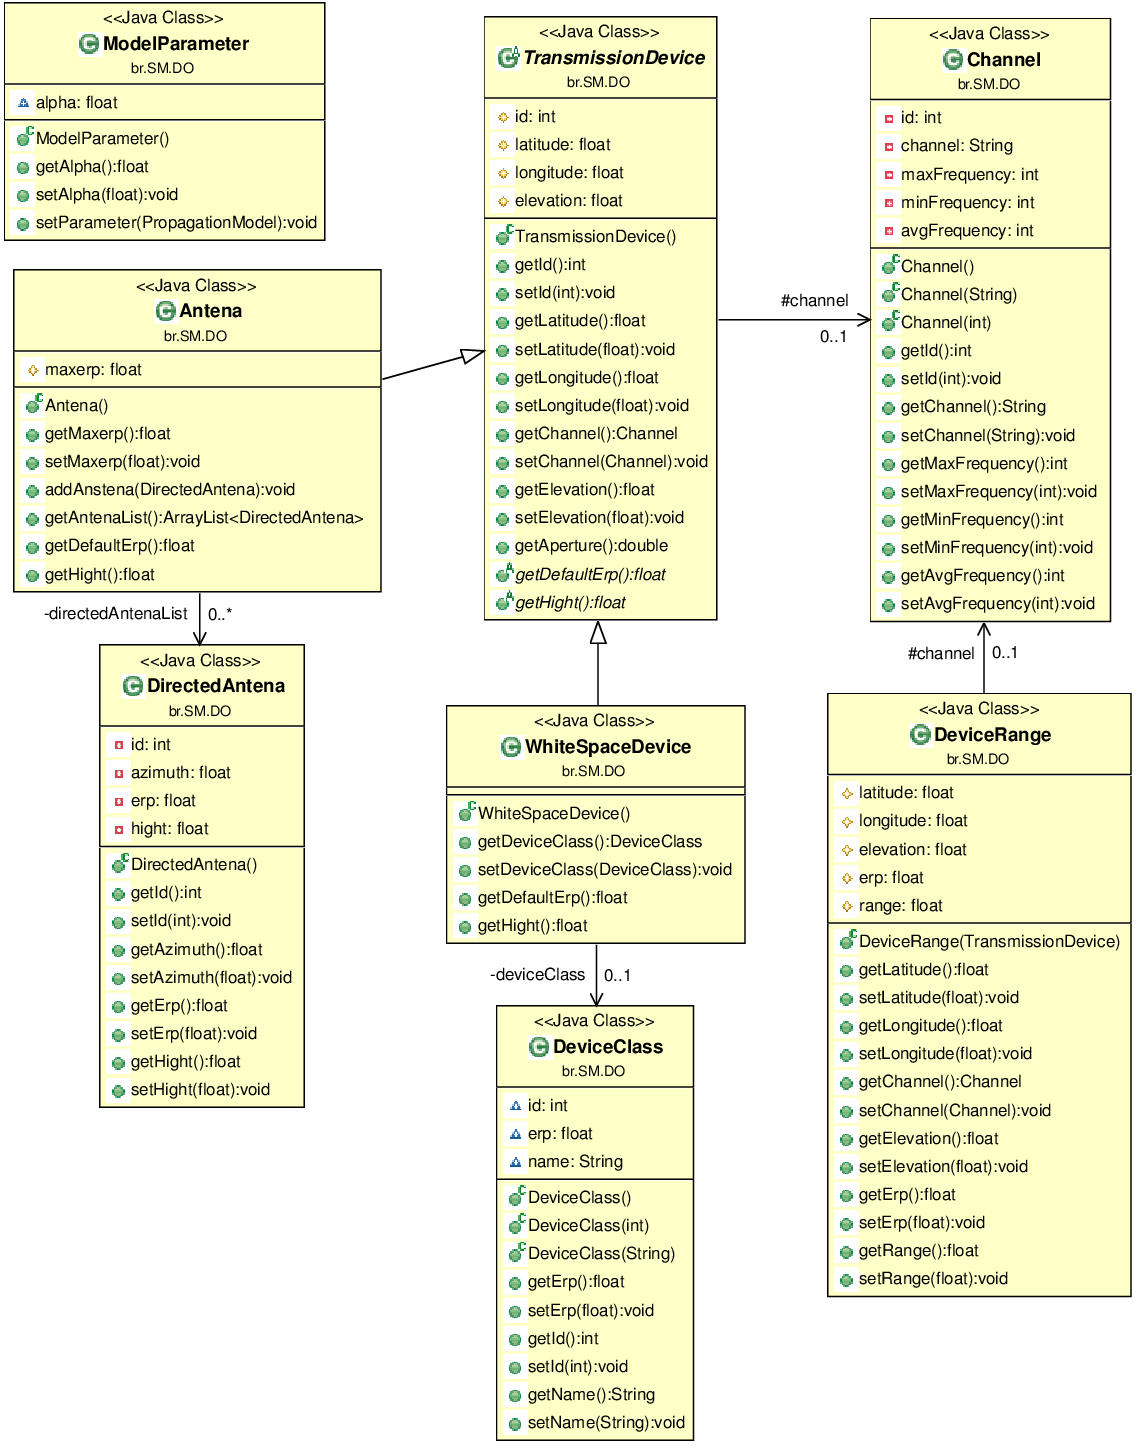
\includegraphics[width=1.0\textwidth]{figs/do}
%\caption[Classes de Dados (DO).]
%{Classes de dados.}
%\label{fig:DO}
%\end{figure} 
%
%O modelo de dados criado no SGBD está indicado no diagrama entidade relacionamento~\ref{fig:ER}.
%
%
%\begin{figure}[htb]
%\centering
%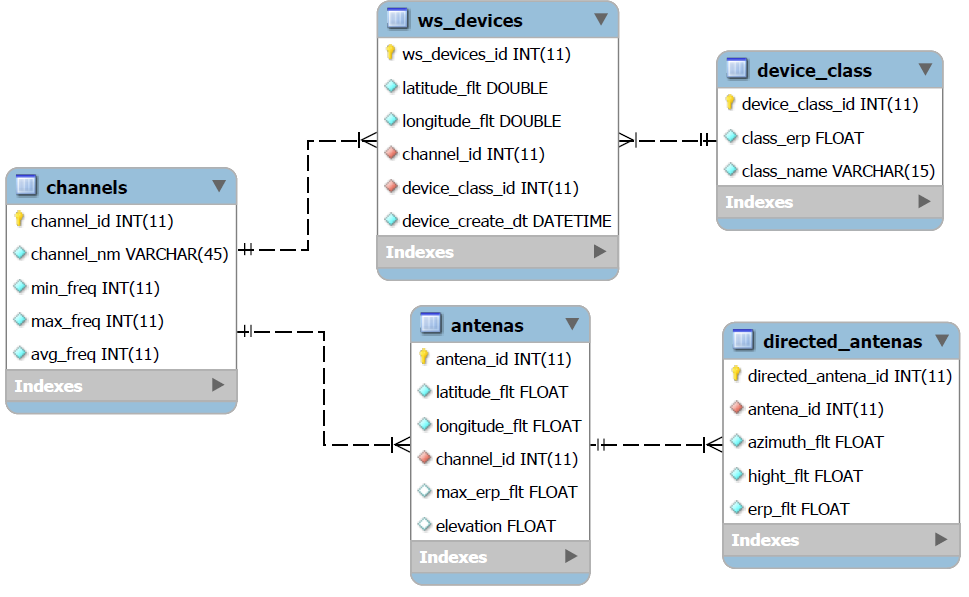
\includegraphics[width=1.0\textwidth]{figs/er}
%\caption[Diagrama Entidade Relacionamento.]
%{Diagrama entidade relacionamento da Base de Dados.}
%\label{fig:ER}
%\end{figure} 
%
%
%
%\subsection{ Data Access Object}
%
%O acesso à base de dados foi desenvolvido usando o padrão de desenvolvimento Data Access Object(DAO).
%\abbrev{DAO}{Data Access Object}
%Nesse padrão todo acesso ao banco de dados é abstraído para as classes DAO. Elas possuem métodos que retornam objetos de dados (DO) de acordo com parâmetros passados. 
%
%Foram desenvolvidas interfaces DAO que possuem todos os métodos necessários para interagir com uma determinada tabela.  Existe, também, a classe \textit{BasicMYSQLDao} que é responsável por gerenciar a conexão com a base de dados criada. Uma classe DAO, como a \textit{AntenaMYSQLDao}, deve herdar a interface correspondente (\textit{AntenaDao}) e estender a\textit{BasicMYSQLDao}. Esse exemplo é retratado na figura~\ref{fig:antenadao}.
%
%\begin{figure}[htb]
%\centering
%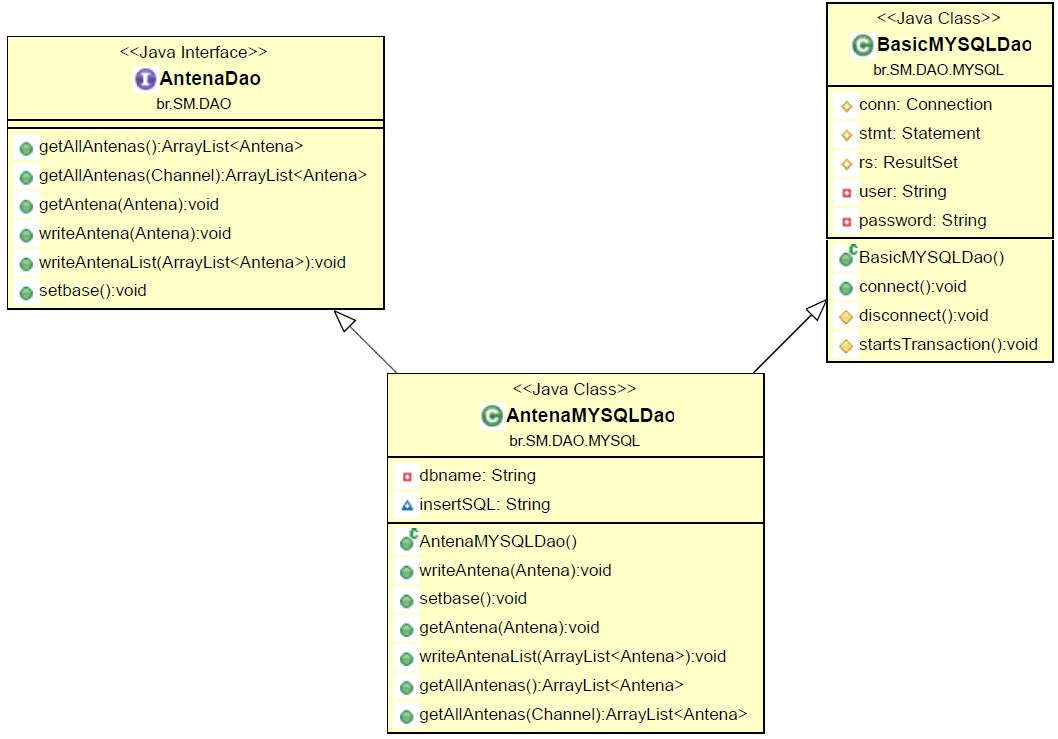
\includegraphics[width=1.0\textwidth]{figs/dao}
%\caption[Exemplo da classe \textit{AntenaMYSQLDao}.]
%{Classe AntenaMYSQLDao.}
%\label{fig:antenadao}
%\end{figure}
%
%
%\subsection{Implementação}
%
%Além das classes DAO, foi desenvolvido uma interface cujo único objetivo é acionar a classe que herde o \textit{RawDataManager}. A ideia é segregar funções.
%
%As classes mencionadas na seção anterior têm apenas uma preocupação, gerar uma lista com as informações que devem ser incluídas na base. Já a interface \textit{SpectrumAvailabilityManager} recebe essa lista e aciona as classes DAO necessárias, de modo a incluir essas informações na base de dados.
%
%A figura~\ref{fig:sm} representa as classes desse módulo.
%
%\begin{figure}[htb]
%\centering
%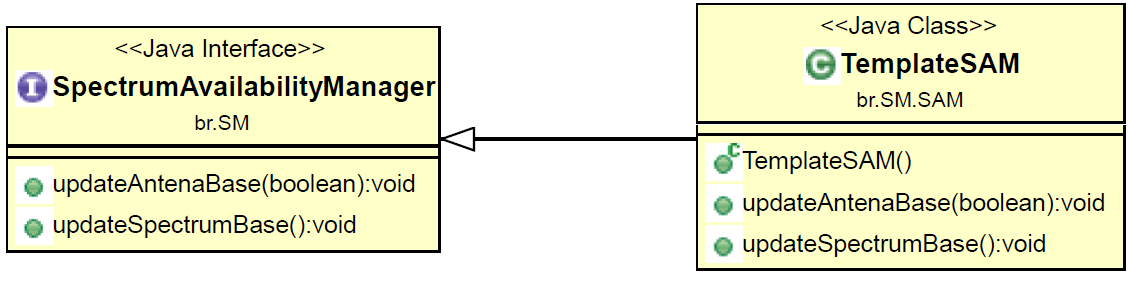
\includegraphics[width=1.0\textwidth]{figs/sm}
%\caption[Diagrama de classes para montar a base de dados.]
%{Diagramas de classe para montar a base de dados.}
%\label{fig:sm}
%\end{figure}
%
%
%\subsection{Extensão}
%
%Para modificar a base de dados utilizada, bem como realizar mudanças no modelo de dados, como modificar de nomes de campos ou da base, basta alterar as classes DAO do MYSQL. Devem ser construídas classes DAO para o SGBD que for utilizado. As classes criadas para o MYSQL podem ser tomadas como exemplo.
%
%As classes DAO implementadas estão representadas na figura~\ref{fig:mysqldao}.
%
%\begin{figure}[htb]
%\centering
%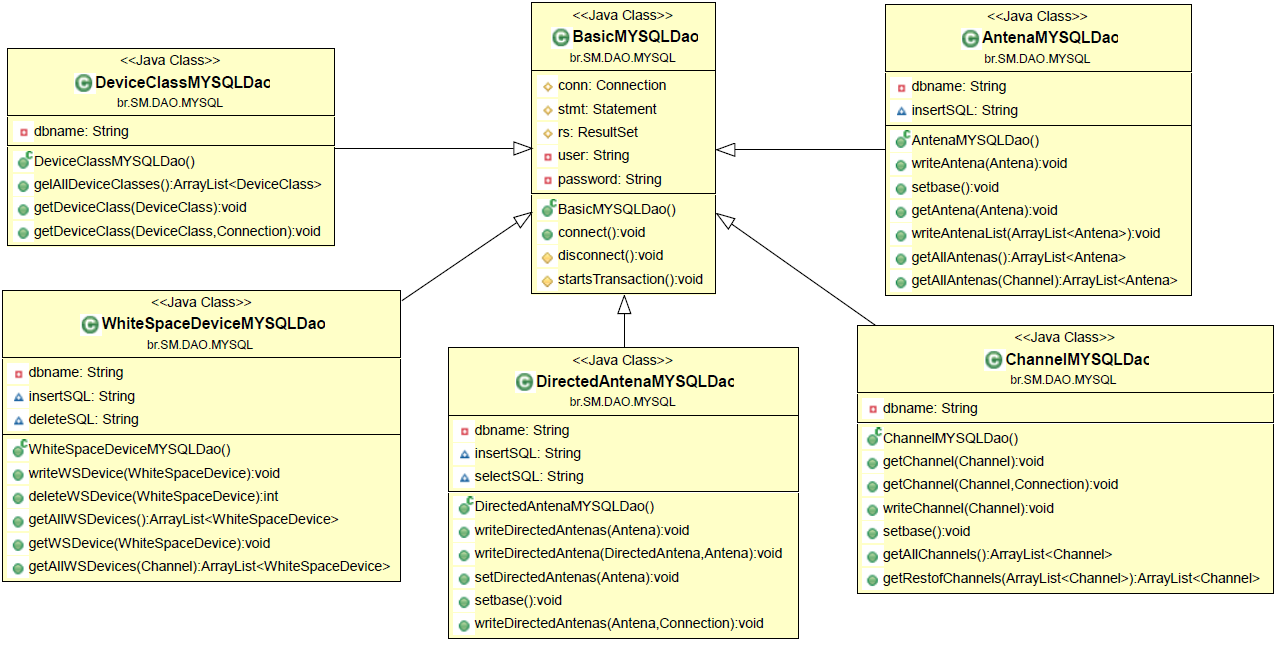
\includegraphics[width=1.0\textwidth]{figs/mysqldao}
%\caption[Diagrama de classes DAO do MYSQL.]
%{Classe DAO do MYSQL.}
%\label{fig:mysqldao}
%\end{figure}
%
%\FloatBarrier
%
%A classe \textit{TemplateSAM}, a princípio, já realiza todas as funções necessárias para montar a base de dados com as informações obtidas da ANATEL e não precisa ser alterada.
%
%\subsection{Canais de transmissão}
%
%As informações referentes aos canais de transmissão utilizados pelas antenas também foram retiradas do site da ANATEL~\cite{canaliza}, e incluídas manualmente na base. As informações utilizadas estão na tabela~\ref{table:tabcanal}.
%
%\begin{center}
%\begin{longtable}{cccc}
%
%\caption[Informações sobre os canais de transmissão.]
%{Tabela obtida do site da ANATEL~\cite{canaliza}}
%\label{table:tabcanal} \\
%
%\hline \multicolumn{1}{|c|}{\textbf{Canal}} & \multicolumn{1}{c|}{\textbf{ Frequência Mínima}} & \multicolumn{1}{c|}{\textbf{Frequência Média}}  & \multicolumn{1}{c|}{\textbf{Frequência Máxima}} \\ \hline 
%\endfirsthead
%
%\multicolumn{4}{c}%
%{{\bfseries \tablename\ \thetable{} -- continuação}} \\
%\hline 
%\multicolumn{1}{|c|}{\textbf{Canal}} &
%\multicolumn{1}{c|}{\textbf{Frequência Mínima}} &
%\multicolumn{1}{c|}{\textbf{Frequência Média }} &
%\multicolumn{1}{c|}{\textbf{Frequência Máxima}} \\ \hline 
%\endhead
%
%\hline 
%\endfoot
%
%\hline \hline
%\endlastfoot
%
%2 & 54 & 57 & 60 \\ 
%3 & 60 & 63 & 66 \\ 
%4 & 66 & 69 & 72 \\ 
%5 & 76 & 79 & 82 \\ 
%6 & 82 & 85 & 88 \\ 
%7 & 174 & 177 & 180 \\ 
%8 & 180 & 183 & 186 \\ 
%9 & 186 & 189 & 192 \\ 
%10 & 192 & 195 & 198 \\ 
%11 & 198 & 201 & 204 \\ 
%12 & 204 & 207 & 210 \\ 
%13 & 210 & 213 & 216 \\ 
%14 & 470 & 473 & 476 \\ 
%15 & 476 & 479 & 482 \\ 
%16 & 482 & 485 & 488 \\ 
%17 & 488 & 491 & 494 \\ 
%18 & 494 & 497 & 500 \\ 
%19 & 500 & 503 & 506 \\ 
%20 & 506 & 509 & 512 \\ 
%21 & 512 & 515 & 518 \\ 
%22 & 518 & 521 & 524 \\ 
%23 & 524 & 527 & 530 \\ 
%24 & 530 & 533 & 536 \\ 
%25 & 536 & 539 & 542 \\ 
%26 & 542 & 545 & 548 \\ 
%27 & 548 & 551 & 554 \\ 
%28 & 554 & 557 & 560 \\ 
%29 & 560 & 563 & 566 \\ 
%30 & 566 & 569 & 572 \\ 
%31 & 572 & 575 & 578 \\ 
%32 & 578 & 581 & 584 \\ 
%33 & 584 & 587 & 590 \\ 
%34 & 590 & 593 & 596 \\ 
%35 & 596 & 599 & 602 \\ 
%36 & 602 & 605 & 608 \\ 
%38 & 614 & 617 & 620 \\ 
%39 & 620 & 623 & 626 \\ 
%40 & 626 & 629 & 632 \\ 
%41 & 632 & 635 & 638 \\ 
%42 & 638 & 641 & 644 \\ 
%43 & 644 & 647 & 650 \\ 
%44 & 650 & 653 & 656 \\ 
%45 & 656 & 659 & 662 \\ 
%46 & 662 & 665 & 668 \\ 
%47 & 668 & 671 & 674 \\ 
%48 & 674 & 677 & 680 \\ 
%49 & 680 & 683 & 686 \\ 
%50 & 686 & 689 & 692 \\ 
%51 & 692 & 695 & 698 \\ 
%52 & 698 & 701 & 704 \\ 
%53 & 704 & 707 & 710 \\ 
%54 & 710 & 713 & 716 \\ 
%55 & 716 & 719 & 722 \\ 
%56 & 722 & 725 & 728 \\ 
%57 & 728 & 731 & 734 \\ 
%58 & 734 & 737 & 740 \\ 
%59 & 740 & 743 & 746 \\ 
%60 & 746 & 749 & 752 \\ 
%61 & 752 & 755 & 758 \\ 
%62 & 758 & 761 & 764 \\ 
%63 & 764 & 767 & 770 \\ 
%64 & 770 & 773 & 776 \\ 
%65 & 776 & 779 & 782 \\ 
%66 & 782 & 785 & 788 \\ 
%67 & 788 & 791 & 794 \\ 
%68 & 794 & 797 & 800 \\ 
%69 & 800 & 803 & 806 \\ 
%
%\end{longtable}
%\end{center}
%
%
%Para os cálculos descritos na seção seguinte, foi utilizado o valor de frequência média.
%
%\section{Determinação do White Space}
%
%A disponibilidade de canais é determinada aplicando modelos de propagação nas antenas contidas na base gerada a partir das informações da ANATEL. 
%
%\subsection{Algoritmo}
%
%Assume-se um dispositivo \textit{x} cujas latitude \textit{lat} e longitude \textit{lng} determinam sua localização no planeta Terra. Todas as antenas na base devem ser percorridas, de forma a determinar em quais delas o dispositivo não interfere, como definido na equação~\ref{interfere}. Os seguintes modelos de propagação foram implementados, para determinar o alcance da antena e de um possível dispositivo:
%
%\begin{itemize}
%\item Free Space
%\item Two Ray Ground
%\item Log Distance
%\end{itemize}
%
%A definição e formulação de cada um deles, mencionadas a seguir, foi retirada de RAPPAPORT~\cite{rapapport}.
%
%Como o sistema armazena informação de reserva de canais, além de verificar se \textit{x} interfere com as antenas da base,  deve ser verificado, também, a condição de interferência com outros dispositivos secundários.
%
%\subsubsection{Definições Gerais}
%
%O objetivo dos modelos implementados é determinar a qual distância da antena seu sinal se atenua a ponto que a relação sinal/ruído se torna igual a 10dB. Além disso, deve ser determinada a distância necessária para que a potência emitida por um possível US se atenue até chegar ao valor do ruído de fundo.
%
%A relação sinal/ruído é definida:
%
%\begin{align}
%  \label{Sinr} SINR=\frac{P}{I+N}
%\end{align}
%
%Onde \textit{P} é a potência do sinal, \textit{I} é a interferência e \textit{N} é o ruído de fundo .
%
%Como é assumido que a única interferência no ambiente será o ruído de fundo, tem-se então que:
%
%\begin{align}
%  \label{actSinr} SINR=\frac{P}{N}
%\end{align}
%
%O ruído de fundo, em Watts, é definido como:
%
%\begin{align}
%  \label{noise} Noise=kTB
%\end{align}
%
%Aonde \textit{k} é a constante de Boltzman, \textit{T} é a temperatura do ambiente e \textit{B} é a banda em hertz.
%
%Assim, pelas equações~\ref{actSinr} e~\ref{noise} tem-se que a potência mínima do receptor é:
%
%\begin{align}
%  \label{minPot} P_r= SINR \cdot  kTB
%\end{align}
%
%O valor da relação sinal/ruído deve ser convertido para W de forma a facilitar os cálculos. Dessa forma:
%
%\begin{align}
%  \label{SinrW} 10= 10 log_{10} (SINR_W)
%\end{align}
%
%De modo que a potência do sinal emitido pela antena em seu alcance máximo será:
%
%\begin{align}
%  \label{minPotAnt} P_{a}= 10kTB
%\end{align}
%
% No entanto, o dispositivo que utiliza o WS não pode interferir com os receptores da antena. Dessa forma, seu sinal deve ser atenuado até atingir o valor do ruído de fundo. Assim sendo, a relação sinal/ruído deve ser de 0dB. De modo que podemos determinar a potência no alcance máximo do dispositivo como sendo:
%
%\begin{align}
%  \label{minPotDev} P_{d}=  kTB
%\end{align}
%
%\subsubsection{Free Space}
%
%O modelo de propagação Free Space admite que o transmissor e o receptor possuem um caminho em linha reta, sem obstruções entre si. Esse modelo é bem simples e sua aplicação resulta em alcances muito superiores aos que eles realmente são. Sua implementação serviu como base para os outros modelos. Ele foi desenhado na figura~\ref{fig:freespaces}.
%
%\begin{figure}[htb]
%\centering
%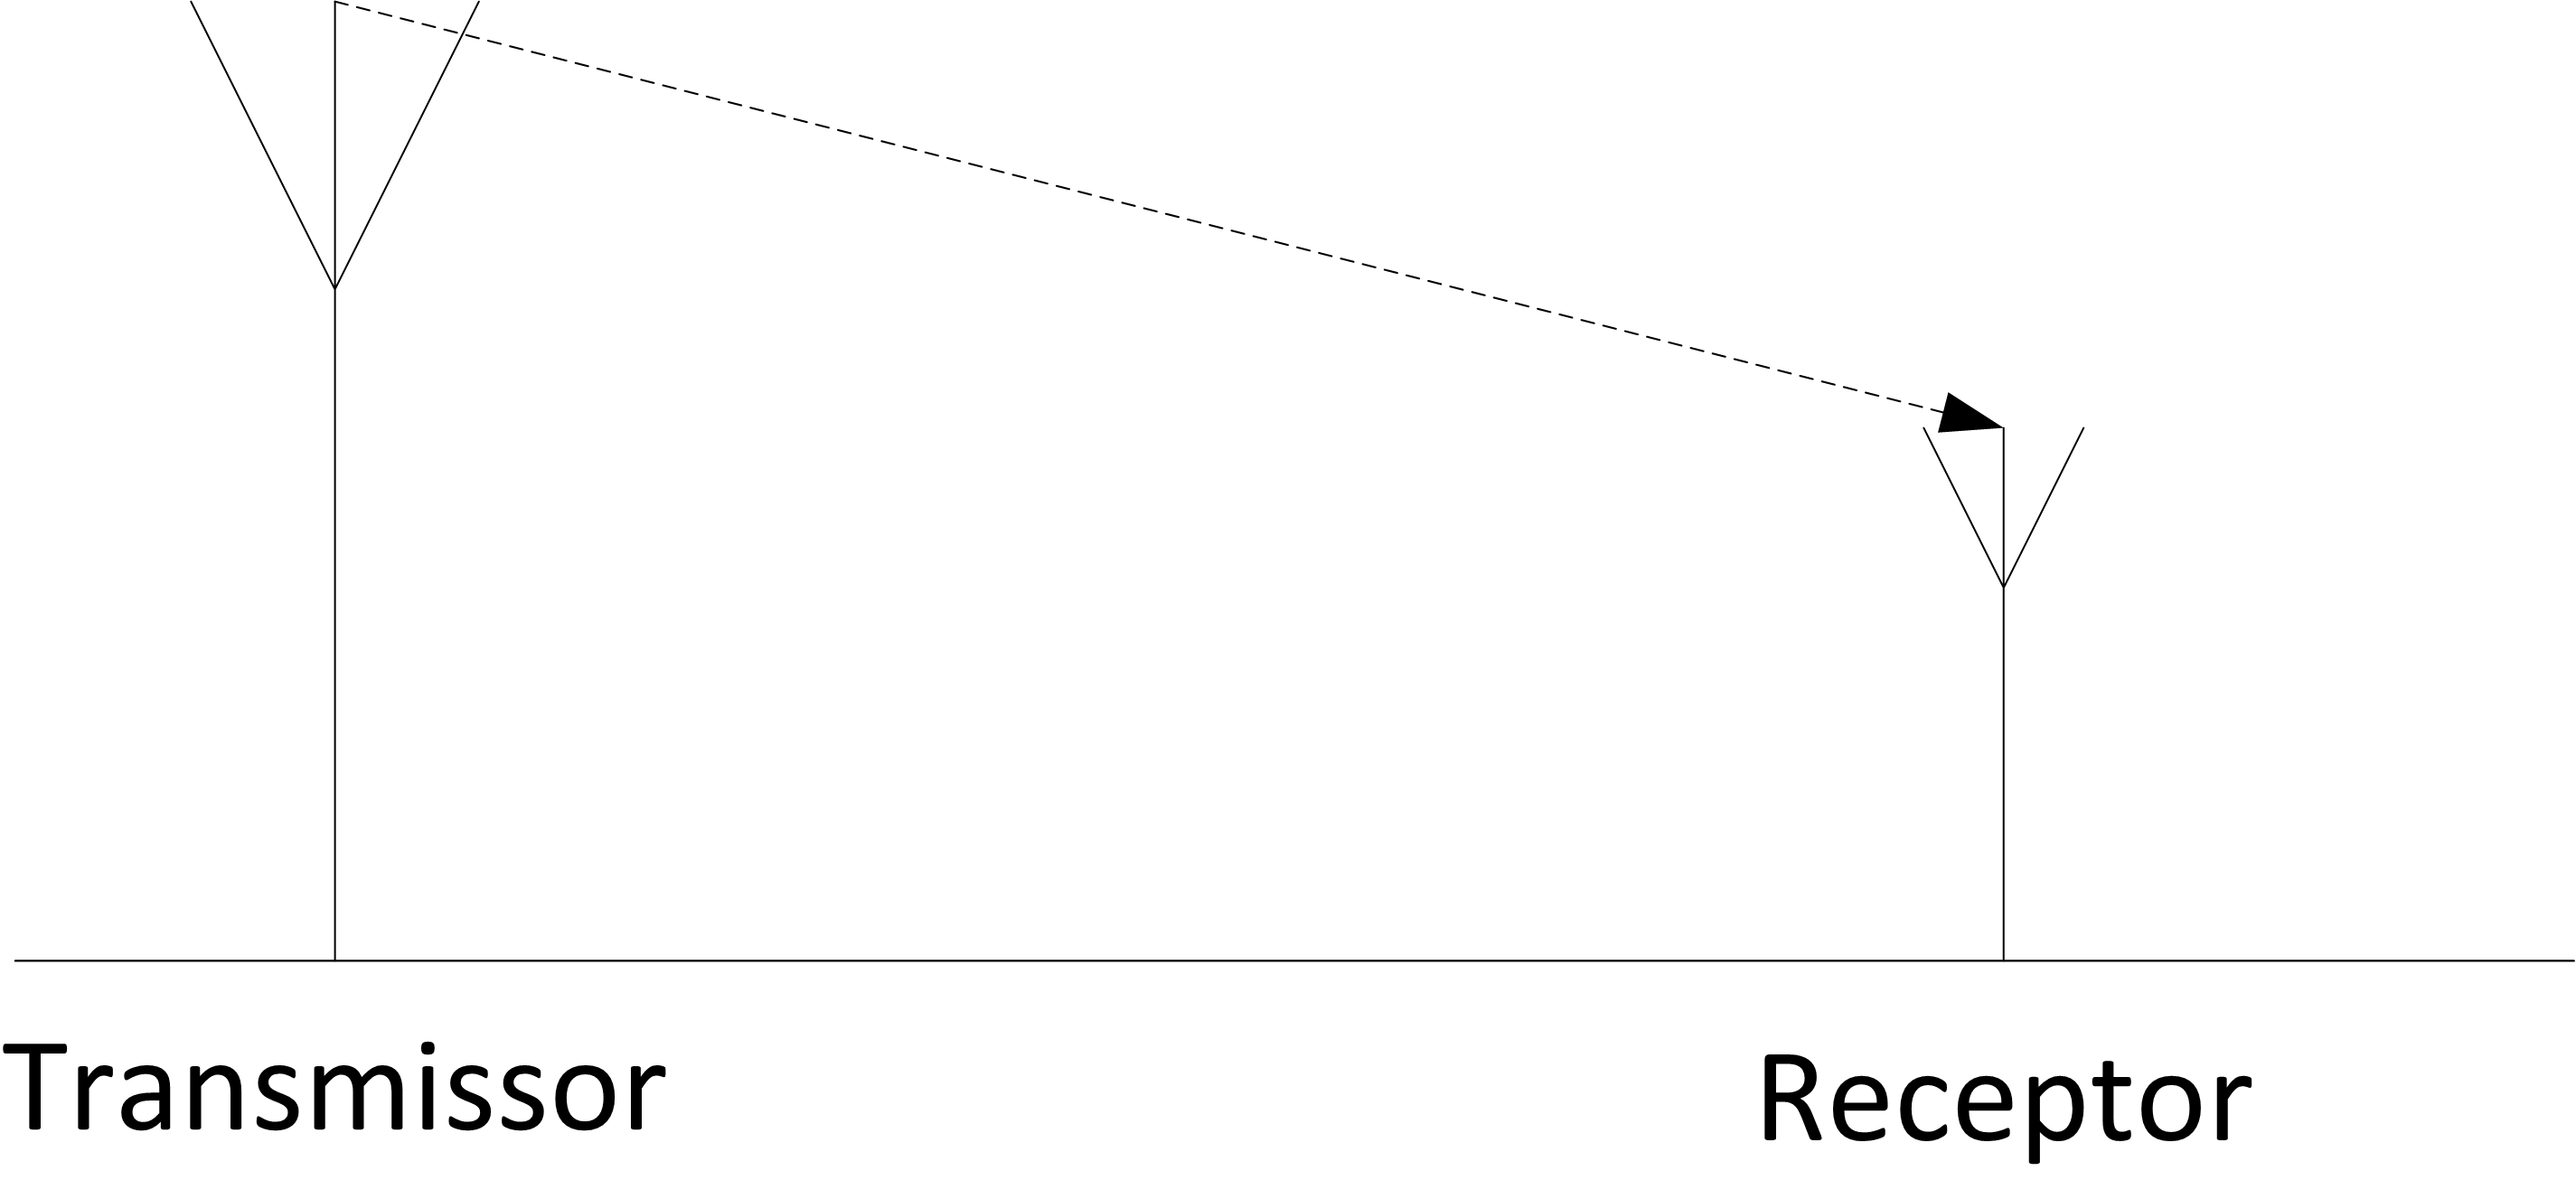
\includegraphics[width=0.8\textwidth]{figs/freespaces}
%\caption[Modelo de propagação Free Space.]
%{Modelo de propagação Free Space.}
%\label{fig:freespaces}
%\end{figure}
%
%A potência recebida pelo receptor quando o transmissor se encontra a uma distância \textit{d} é definida~\cite{rapapport} como: 
%
%\begin{align}
%  \label{potfree} P_r(d) =\frac{ P_tG_tG_r\lambda^{2}}{(4\pi)^{2}d^{2}L}
%\end{align}
%
%\begin{math}G_t\end{math} e \begin{math}G_r\end{math} são os ganhos do transmissor e receptor respectivamente. Foi assumido que a potência indicada pela ANATEL é, na verdade, \begin{math}P_tG_t\end{math}, enquanto \begin{math}G_r\end{math} foi desconsiderado.
%
%\begin{align}
%  \label{ganho} G_r = 1
%\end{align}
%
%\textit{L} representa o fator de perda não relacionado ao modelo de propagação. L também foi desconsiderado.
%
%\begin{align}
%  \label{loss} L = 1
%\end{align}
%
%\begin{math}\lambda\end{math} é referente a frequência utilizada para transmissão, onde \textit{c} é a velocidade da luz em m/s e \textit{f} é a frequência utilizada em Hz.
%
%\begin{align}
%  \label{lambda}\lambda=\frac{c}{f}
%\end{align}
%
%Assim sendo, determina-se o alcance de uma antena no modelo de Free Space pelas equações~\ref{potfree} e~\ref{minPotAnt}:
%
%\begin{align}
%  \label{dFreeAnt} d_1 = \sqrt{\frac{P_t\lambda^{2}}{10kTBL(4\pi)^{2}}}
%\end{align}
%
%De maneira análoga, o alcance de um US pode ser determinado pelas equações~\ref{potfree} e~\ref{minPotDev}:
%
%\begin{align}
%  \label{dFreeDev} d_2 = \sqrt{\frac{P_t\lambda^{2}}{kTBL(4\pi)^{2}}}
%\end{align}
%
%\subsubsection{Two Ray Ground}
%
%O modelo Two Ray Ground, ou de Reflexão no Chão, assume a possibilidade de reflexão do sinal emitido. O sinal enviado pelo transmissor, além de alcançar o receptor por uma linha direta como no Free Space, vai refletir no chão e chegar ao receptor. Dessa forma, dois raios chegam ao receptor: o refletido e o não refletido. Como indicado na figura~\ref{fig:tworay}.
%
%\begin{figure}[htb]
%\centering
%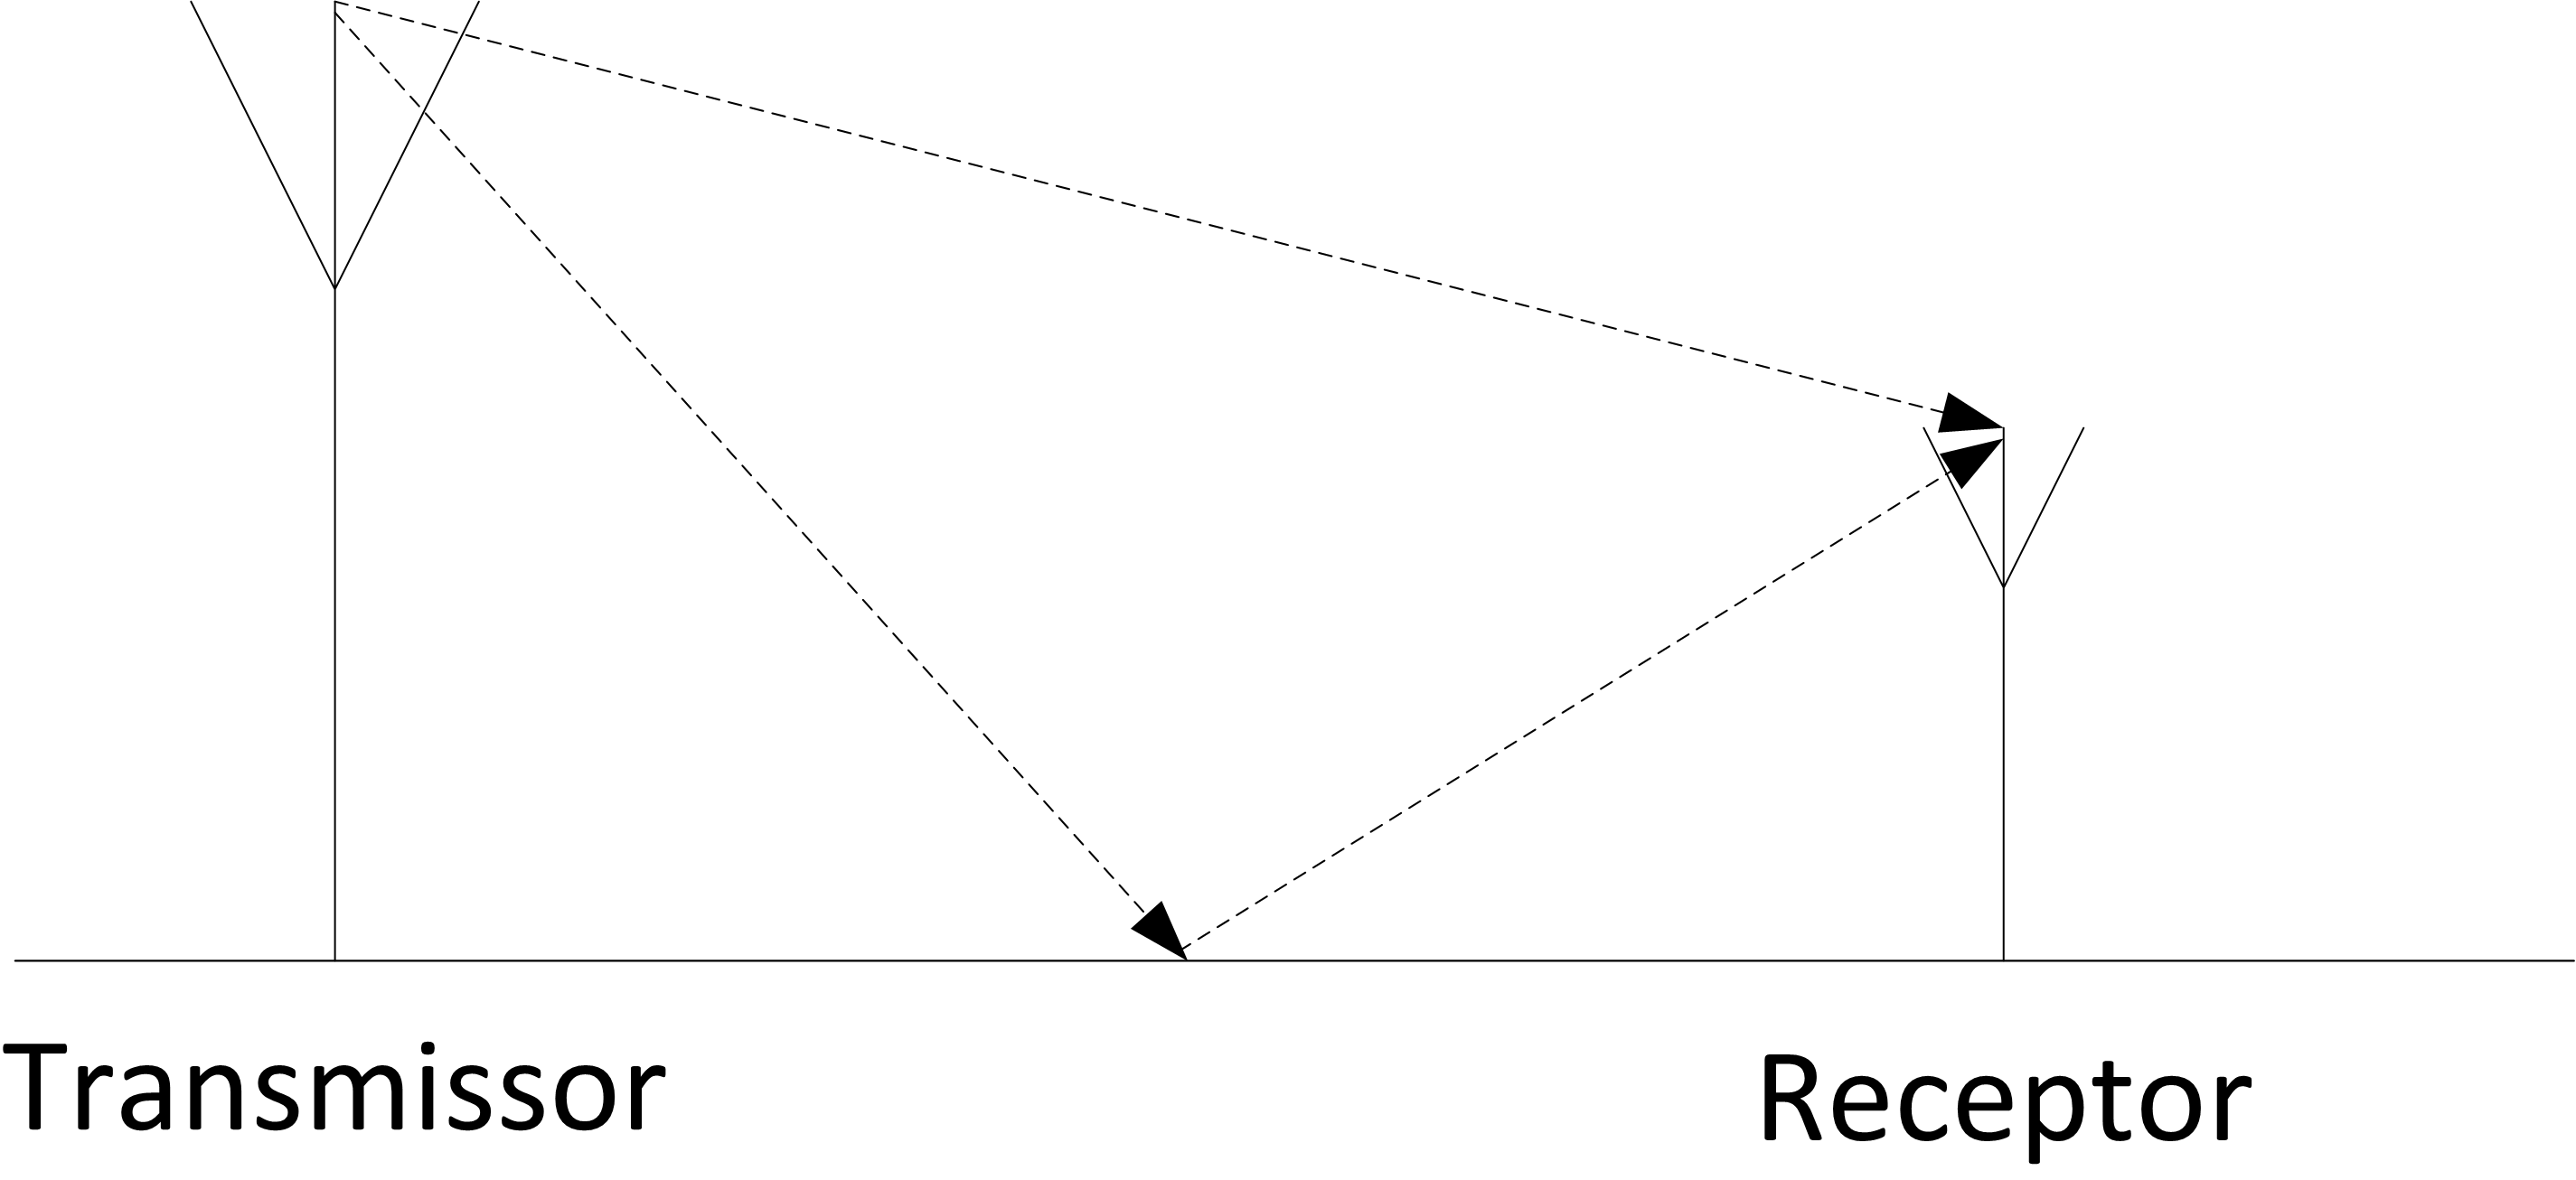
\includegraphics[width=0.8\textwidth]{figs/tworay}
%\caption[Modelo de propagação Two Ray Ground.]
%{Modelo de propagação Two Ray Ground.}
%\label{fig:tworay}
%\end{figure}
%
%
%A potência recebida pelo receptor quando o transmissor se encontra a uma distância \textit{d} é definida~\cite{rapapport} como: 
%
%\begin{align}
%  \label{pottworay} P_r(d) = P_tG_tG_r\frac{h_t^{2}h_r^{2}}{d^4}
%\end{align}
%
%Onde \begin{math}h_t\end{math} é a altura da antena transmissora e \begin{math}h_r\end{math} é a altura da antena do receptor em metros. Foi assumida uma altura de 2 metros para casos onde não foi possível determinar a altura do dispositivo.
%
%Assim, assumindo a equação~\ref{ganho}, temos, pelas equações~\ref{pottworay} e~\ref{minPotAnt} o alcance de uma antena no modelo Two Ray Ground:
%
%\begin{align}
%  \label{dTwoRayAnt} d_1 = \sqrt[4]{\frac{P_th_t^{2}h_r^{2}}{10kTB}}
%\end{align}
%
%De maneira análoga, o alcance de um US pode ser determinado pelas equações~\ref{potfree} e~\ref{minPotDev}:
%
%\begin{align}
%  \label{dTwoRayDev} d_2 = \sqrt[4]{\frac{P_th_t^{2}h_r^{2}}{kTB}}
%\end{align}
%
%
%\subsubsection{Log Distance}
%
%O modelo de propagação Log Distance assume que a potência transmitida por uma antena decai logaritmicamente em relação à distância. Dois fatores principais entram em cena, a perda ocorrida a uma distância muito pequena, e a taxa de decaimento.
%
%\begin{math}L_0\end{math} determina a perda ocorrida a uma distância muito pequena. Foi considerado a distância \begin{math}d_0\end{math} como sendo 1 metro. Essa perda foi calculada no modelo Free Space:
%
%\begin{align}
%  \label{L0} L_0 = \left( \frac{4\pi w}{c}\right)^{2}
%\end{align}
%
%Onde \begin{math}w\end{math} é o comprimento de onda da freqência utilizada e \begin{math}c\end{math} é a velocidade da luz em metros.
%
%O modelo foi simplificado de forma que o alcance de uma antena é representado por:
%
%\begin{align}
%  \label{dLogDistAnt} d_1 = \sqrt[\gamma]{\frac{d_0^{\gamma}10^{\frac{-L_0}{10}}  P_t}{10kTB}}
%\end{align}
%
%De maneira análoga, o alcance de um US é representado por:
%\begin{align}
%  \label{dLogDistDev} d_2 = \sqrt[\gamma]{\frac{d_0^{\gamma}10^{\frac{-L_0}{10}}  P_t}{kTB}}
%\end{align}
%
%\begin{math}\gamma \end{math} representa um fator de perda que geralmente recebe valores de 2 a 6. Foi escolhido 3 como sendo valor padrão.
%
%\subsubsection{Constantes}
%
%As seguintes constantes foram assumidas para os cálculos descritos:
%
%\begin{itemize}
%\item k =\begin{math}1380\cdot 10^{-23}\end{math}  mW
%\item T = 290 K
%\item B = 6 MHz
%\item c = 299792458 m/s
%\end{itemize}
%
%
%\subsection{Implementação}
%
%Foi desenvolvida a classe abstrata \textit{PropagationModel} que define as constantes e alguns métodos básicos para todos modelos de propagação. Foram geradas classes para cada um dos modelos de propagação descritos a cima. Eles implementam o método \textit{maxDistance} que indica o alcance de um determinado dispositivo. A figura~\ref{fig:models} representa as classes criadas.
%
%\begin{figure}[htb]
%\centering
%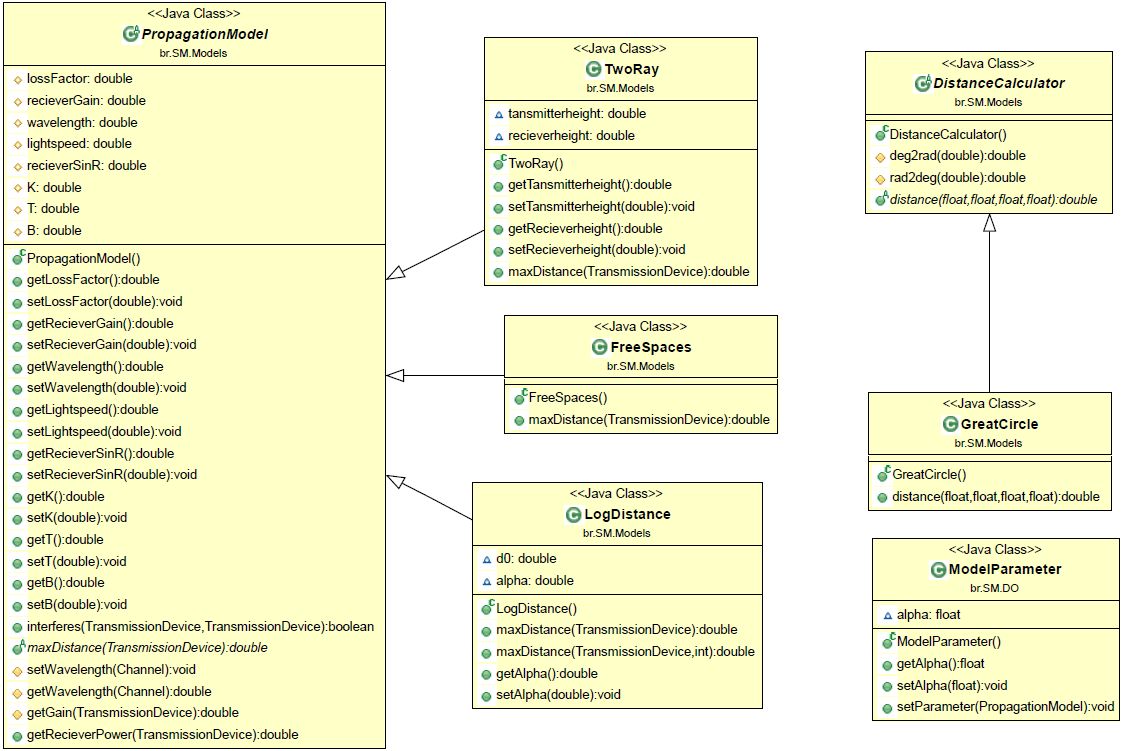
\includegraphics[width=1.0\textwidth]{figs/models}
%\caption[\textit{Diagrama de classes dos modelos de propagação desenvolvidos}.]
%{Diagrama de classes dos modelos de propagação desenvolvidos.}
%\label{fig:models}
%\end{figure} 
%
%A classe \textit{PropagationModel} possui o método \textit{interferes} que indica se 2 dispositivos estão em condição de interferência.
%
%O modelo de propagação utilizado é indicado ao chamar a sua classe Factory \textit{PropagationModelFactory}.
%
%A classe \textit{ModelParameter} possui uma lista com todos os parâmetros utilizados pelos modelos. O Construtor dessa classe atribui a esses parâmetros seus valores padrões. Sempre que for necessário indicar um parâmetro a um modelo isto é feito utilizando essa classe.
%
%\subsection{Extensão}
%
%Para criar novos modelos de propagação basta criar classes que estendam a \textit{PropagationModel} e incluir seus possíveis parâmetros na classe \textit{ModelParameter}.
%
%\section{Web Service Desenvolvido}
%
%
%Web Services são uma maneira de disponibilizar um serviço cliente servidor em uma rede. Uma mensagem é enviada do cliente ao servidor, que executa o serviço e envia uma mensagem de resposta ao cliente. A interface definida pelo servidor deve ser indicada ao cliente, bem como o formato de resposta utilizado.
%
%O Web Service desenvolvido tem dois objetivos. O primeiro é de prestar o serviço de disponibilidade de canais no WS, como descrito no PAWS. O segundo é de tornar disponível todas as informações contidas na base desenvolvida. Foi criado, então, um serviço para cada tipo de item disponível:
%
%\begin{itemize}
%\item Canal
%\item Antena
%\item Dispositivo Secundário
%\end{itemize}
%
%Além disso, é possível determinar o modelo de propagação que será utilizado pelo servidor para realizar os devidos cálculos.
%
%
%\subsection{REST}
%
%O Web Service foi desenvolvido no modelo REST~\cite{restful}. O seu conceito básico é que a base consiste de recursos, cada um com um Uniform Resource Identifier (URI)
%\abbrev{URI}{Uniform Resource Identifier}
%específico. Os URIs consistem de URLs que são alcançáveis por pedidos HTTP. Pode-se, então, interagir com toda base enviando pedidos HTTP.
%
%Existem quatro tipos de pedido HTTP que podem ser utilizados:
%
%\begin{itemize}
%\item GET - utilizado para buscar um recurso
%\item POST - utilizado para alterar o valor de um recurso
%\item PUT - utilizado para alterar o valor de um recurso
%\item DELETE - utilizado para excluir um recurso
%\end{itemize}
%
%O POST e o PUT possuem basicamente a mesma função. A especificação do HTTP~\cite{RFC2616} define que o PUT deve ser utilizado quando um novo recurso é criado na base, enquanto o POST modifica um recurso já existente. No entanto, o PUT também pode ser usado para modificar um recurso já existente. Dessa forma, apenas o PUT foi utilizado no sistema desenvolvido.
%
%Praticamente não existe uma diferença entre um Web Service REST e outro em SOAP, por exemplo. Os dois podem prover os mesmos serviços. No entanto, outros Web Services geralmente precisam preparar a mensagem que será enviada ao servidor. Já no REST as mensagens são simples pedidos de HTTP, com os parâmetros estando, muitas das vezes, nos próprios parâmetros da URL.
%
%Não existe uma forma padrão para a resposta do servidor ao cliente. Entretanto, isso muitas vezes é feito via JSON ou XML, já que estes formatos apresentam uma forma mais estruturada. No servidor desenvolvido o formato de resposta escolhido foi o XML.
%
%Pode-se resumir o funcionamento do servidor REST desenvolvido da seguinte maneira:
%
%\begin{itemize}
%\item O cliente faz um pedido HTTP em uma URL do servidor
%\item O servidor identifica qual recurso essa URL serve
%\item O servidor processa o pedido e retorna o recurso
%\item O cliente recebe a resposta do servidor no formato XML
%\end{itemize}
%
%A escolha pelo REST, em detrimento do JSON-RPC se deu pela sua maior facilidade de testes. Como o serviço REST é alcançado por um pedido HTTP, pode-se usar qualquer browser da internet para verificá-lo.
%
%\subsection{Implementação}
%
%Os serviços prestados pela base foram indicados nas interfaces API. As classes que herdam essa API implementam os métodos que serão utilizados remotamente. Essas classes serão descritas na seção API.
%
%Foi utilizada a biblioteca Restlet~\cite{restlet} para a criação do Web Service. Aqui foram definidas outras classes que apenas invocam as classes mencionadas acima. Essa segregação foi feita para poder dissociar o serviço prestado do tipo de Web Service criado. 
%
%Dessa forma, caso seja preciso modificar o Web Service de REST para JSON-RPC, isso pode ser feito sem que seja necessário redefinir os métodos da API. Apenas as classes de interface com o cliente vão precisar ser modificadas.
%
%A API definida pode ser separada em duas finalidades. Existe a API padrão, que realiza todos os cálculos usando o modelo de propagação Log Distance, e uma API para testes, onde o modelo a ser utilizado pode ser escolhido, bem como suas constantes alteradas. A princípio um dispositivo só precisaria utilizar a API padrão. A API de testes é utilizada apenas para realizar testes com a base, já que dois dispositivos que utilizem modelos de propagação diferentes para seus cálculos acabam recebendo informações desconexas.
%
%\subsection{Extensão}
%
%O tipo de Web Service utilizado pode ser facilmente alterado, basta que as classes referentes ao Web Service invoquem as classes API. 
%
%Novas funcionalidades também podem ser desenvolvidas. Elas devem ser colocadas em novas Interfaces API ou modificar as interfaces existentes.
%
%\subsection{API}
%
%De forma a padronizar a resposta do serviço foi criada a classe \textit{DeviceRange}, indicada na figura~\ref{fig:devicerange}. Essa classe possui todas as informações básicas de um dispositivo de transmissão:
%
%\begin{itemize}
%\item Latitude do dispositivo -- \textit{DeviceRange.latitude}
%\item Longitude do dispositivo -- \textit{DeviceRange.longitude}
%\item Canal utilizado pelo dispositivo -- \textit{DeviceRange.channel}
%\item Elevação do dispositivo -- \textit{DeviceRange.elevation}
%\item Potência do dispositivo -- \textit{DeviceRange.erp}
%\item Alcance calculado para o dispositivo -- \textit{DeviceRange.range}
%\end{itemize}
%
%\begin{figure}[htb]
%\centering
%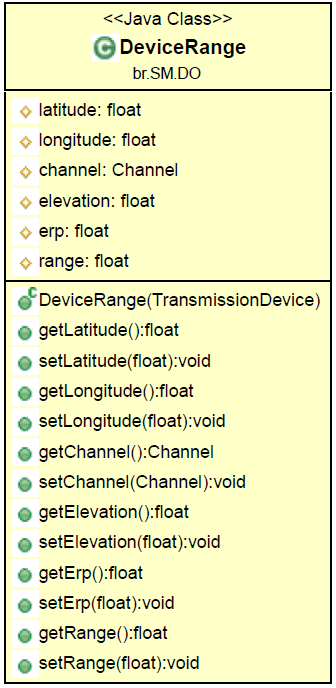
\includegraphics[height=0.4\textheight]{figs/devicerange}
%\caption[\textit{Diagrama da classe \textit{DeviceRange} }.]
%{Diagrama da classe \textit{DeviceRange}.}
%\label{fig:devicerange}
%\end{figure} 
%
%Outra classe utilizada nas respostas é a classe \textit{Channel}, indicada na figura~\ref{fig:channel}. Ela possui as informações básicas sobre um determinado canal de frequência:
%
%\begin{itemize}
%\item Número do canal -- \textit{Channel.channel}
%\item Frequência máxima do canal -- \textit{Channel.maxFrequency}
%\item Frequência mínima do canal -- \textit{Channel.minFrequency}
%\item Frequência média do canal -- \textit{Channel.avgFrequency}
%\end{itemize}
%
%\begin{figure}[htb]
%\centering
%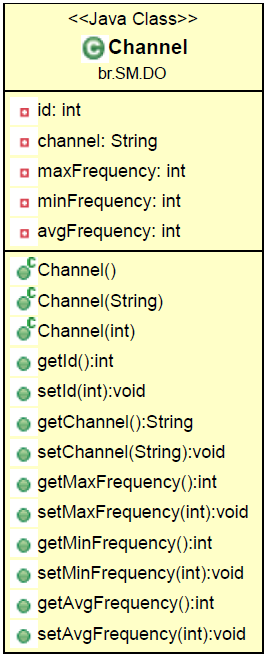
\includegraphics[height=0.4\textheight]{figs/channel}
%\caption[Diagrama da classe \textit{Channel}.]
%{Diagrama da classe \textit{Channel}.}
%\label{fig:channel}
%\end{figure} 
%
%\FloatBarrier
%
%Segue o formato do arquivo XML retornado 
%
%\begin{lstlisting}[language=XML]
%<list>
%  <br.SM.DO.DeviceRange>
%    <latitude>-23.0167</latitude>
%    <longitude>-44.2886</longitude>
%    <channel>
%      <id>24</id>
%      <channel>25</channel>
%      <maxFrequency>542</maxFrequency>
%      <minFrequency>536</minFrequency>
%      <avgFrequency>539</avgFrequency>
%    </channel>
%    <elevation>22.4531</elevation>
%    <erp>1250.0</erp>
%    <range>0.0</range>
%  </br.SM.DO.DeviceRange>
%</list>		
%\end{lstlisting}
%
%\begin{lstlisting}[language=XML]
%<list>
%  <br.SM.DO.Channel>
%    <id>1</id>
%    <channel>2</channel>
%    <maxFrequency>60</maxFrequency>
%    <minFrequency>54</minFrequency>
%    <avgFrequency>57</avgFrequency>
%  </br.SM.DO.Channel>
%</list>	
%\end{lstlisting}
%
%
%Foram desenvolvidas quatro classes de API:
%
%\begin{itemize}
%\item ChannelAPI
%\item AntenaAPI
%\item WSDeviceAPI
%\item TransmissionDeviceAPI
%\end{itemize}
%
%
%\FloatBarrier
%
%\subsubsection{Uso}
%
%Um resumo de utilização da API pode ser descrito como:
%
%
%\begin{itemize}
%\item http://servidor/SAM/devices
%\begin{itemize}
%	\item GET -- Busca todos os dispositivos de transmissão presentes na base;
%\end{itemize}
%\item http://servidor/SAM/devices/location
%\begin{itemize}
%	\item GET -- Busca todos os dispositivos de transmissão presentes na base dada uma localização;
%\end{itemize}
%\item http://servidor/SAM/devices/channel
%\begin{itemize}
%	\item GET -- Busca todos os dispositivos de transmissão presentes na base dado um canal;
%\end{itemize}
%\item http://servidor/SAM/devices/antennas
%\begin{itemize}
%	\item GET -- Busca todas as antenas presentes na base;
%\end{itemize}
%\item http://servidor/SAM/devices/antennas/location
%\begin{itemize}
%	\item GET -- Busca todas as antenas presentes na base dada uma localização;
%\end{itemize}
%\item http://servidor/SAM/devices/antennas/channel
%\begin{itemize}
%	\item GET -- Busca todas as antenas presentes na base dado um canal;
%\end{itemize}
%\item http://servidor/SAM/devices/ws
%\begin{itemize}
%	\item GET -- Busca todos os dispositivos secundários presentes na base;
%	\item PUT -- Cadastra um dispositivo secundário na base;
%	\item DELETE -- Remove um dispositivo secundário na base;
%\end{itemize}
%\item http://servidor/SAM/devices/ws/location
%\begin{itemize}
%	\item GET -- Busca todos os dispositivos secundários na base dada uma localização;
%\end{itemize}
%\item http://servidor/SAM/devices/ws/channel
%\begin{itemize}
%	\item GET -- Busca todos os dispositivos secundários na base dado um canal;
%\end{itemize}
%\item http://servidor/SAM/devices/ws/classes
%\begin{itemize}
%	\item GET -- Busca todos os tipos de dispositivos secundários cadastrados na base;
%\end{itemize}
%\item http://servidor/SAM/channels
%\begin{itemize}
%	\item GET -- Busca todos os canais cadastrados na base;
%\end{itemize}
%\item http://servidor/SAM/channels/available
%\begin{itemize}
%	\item GET -- Busca os canais disponíveis para uso por um determinado dispositivo;
%\end{itemize}
%\end{itemize}
%
%
%
%
%
%
%\subsubsection{ChannelAPI}
%
%
%\begin{figure}[htb]
%\centering
%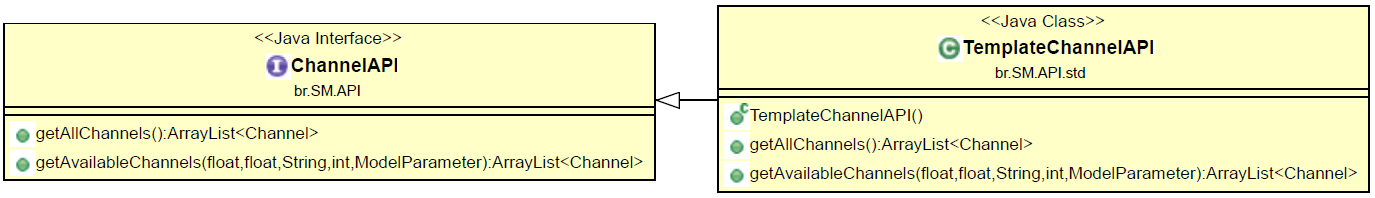
\includegraphics[width=1.0\textwidth]{figs/channelapi}
%\caption[\textit{Diagrama da classe \textit{ChannelAPI} }.]
%{Diagrama da classe \textit{ChannelAPI}.}
%\label{fig:ChannelAPI}
%\end{figure} 
%
%A classe \textit{ChannelAPI}, representada na figura~\ref{fig:ChannelAPI}, define dois métodos:
%
%\begin{lstlisting}
%	public ArrayList<Channel> getAllChannels();
%\end{lstlisting}
%
%Este método retorna uma lista com todos os canais de frequência registrados na base.
%
%Ele é alcançado pela URL \textit{"http://servidor/SAM/channels"}, utilizando o método GET. Esse método não recebe nenhum parâmetro.
%
%A resposta desse método é uma lista de objetos \textit{Channel}, como indicado na seção anterior.
%
%\begin{lstlisting}
%	public ArrayList<Channel> getAvailableChannels(float lat, float lng, String deviceType, int modeltype, ModelParameter par);
%\end{lstlisting}
%
%Este método retorna todos os canais disponíveis para uso em uma determinada posição. Deve ser indicado pelo cliente o tipo de dispositivo que está realizando a busca.
%
%Ele é alcançado pela URL \textit{"http://servidor/SAM/channels/available"}, utilizando o método GET. Pode ser utilizado, também a URL \textit{"http://servidor/SAM/ model/[modelo]/channels/available"} onde \textit{[modelo]} indica o modelo de propagação que será utilizado para o cálculo dos alcances. Podem ser indicados três valores para modelo:
%
%\begin{itemize}
%\item 0 -- Free Space
%\item 1 -- Log Distance
%\item 2 -- Two Ray Ground
%\end{itemize}
%
%Esse método recebe alguns parâmetros, que são submetidos pelo cliente como parâmetros de URL:
%
%\begin{itemize}
%\item \textit{lat} -- A latitude da posição pesquisada. É indicado pelo parâmetro de URL "lat".
%\item \textit{lng} -- A longitude da posição pesquisada. É indicado pelo parâmetro de URL "lng".
%\item \textit{deviceType} -- O tipo de dispositivo que deseja utilizar o WS. É indicado pelo parâmetro de URL "type".
%\item \textit{modeltype} -- O modelo de propagação a ser utilizado. É indicado no corpo da URL. Só utilizado pela API de testes. A API padrão utiliza automaticamente o modelo Log Distance.
%\item \textit{par} -- Constituído de parâmetros específicos para um determinado modelo. Só utilizado pela API de testes. Cada modelo sabe quais parâmetros deve buscar. Para o modelo Log Distance o valor de \begin{math} \alpha \end{math} pode ser indicado pelo parâmetro de URL "alpha" .
%\end{itemize}
%
%\FloatBarrier
%
%Exemplo da URL utilizando a API padrão:
%
%\begin{lstlisting}	
%
%http://localhost:8182/SAM/channels/available?
%	lat=-22.845882&lng=-43.08815&type=INTERNO+BAIXO
%
%\end{lstlisting}
%
%Exemplo da URL utilizando a API de teste:
%
%\begin{lstlisting}			
%
%http://localhost:8182/SAM/model/1/channels/available?
%	lat=-22.845882&lng=-43.08815&type=INTERNO+BAIXO&alpha=2.5
%
%\end{lstlisting}
%
%
%
%A resposta desse método é uma lista de objetos \textit{Channel}, como indicado na seção anterior.
%
%\subsubsection{AntenaAPI}
%
%\begin{figure}[htb]
%\centering
%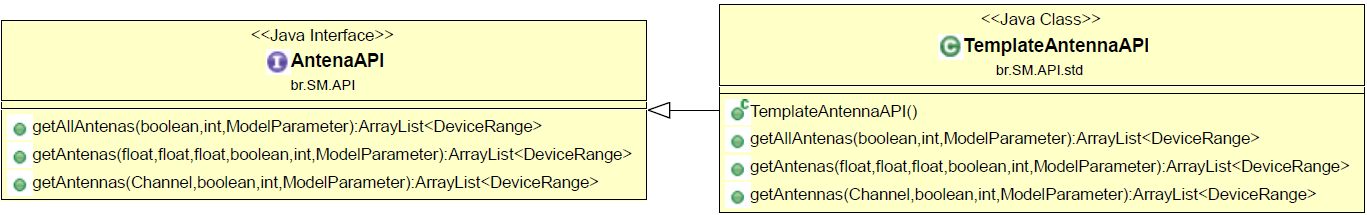
\includegraphics[width=1.0\textwidth]{figs/antenaapi}
%\caption[\textit{Diagrama da classe \textit{AntenaAPI} }.]
%{Diagrama da classe \textit{AntenaAPI}.}
%\label{fig:AntenaAPI}
%\end{figure} 
%
%
%\FloatBarrier
%
%A classe \textit{AntenaAPI}, representada na figura~\ref{fig:AntenaAPI}, define três métodos:
%
%\begin{lstlisting}
%
%	public ArrayList<DeviceRange> getAllAntenas(boolean range, int modeltype, 
%			ModelParameter par);
%
%\end{lstlisting}
%
%Este método retorna uma lista com todas as antenas presentes na base de dados, bem como o seu alcance.
%
%Ele é alcançado pela URL \textit{"http://servidor/SAM/devices/antennas"}, utilizando o método GET. Pode ser utilizado, também a URL \textit{"http://servidor/SAM/ model/[modelo]/devices/antennas"} onde \textit{[modelo]} indica o modelo de propagação que será utilizado para o cálculo dos alcances.
%
%Este método recebe alguns parâmetros, que são submetidos pelo cliente como parâmetros de URL:
%
%\begin{itemize}
%\item \textit{range} -- Um booleano que indica se a API deve calcular o alcance das antenas ou não. É indicado pelo parâmetro de URL "range". Deve ser "true" ou "false". Se nenhum valor for indicado, será utilizado o valor padrão "false".
%\item \textit{modeltype} -- O modelo de propagação a ser utilizado. É indicado no corpo da URL. Só utilizado pela API de testes. A API padrão utiliza automaticamente o modelo Log Distance.
%\item \textit{par} -- Constitui de parâmetros específicos para um determinado modelo. Só utilizado pela API de testes. Cada modelo sabe quais parâmetros deve buscar. Para o modelo Log Distance o valor de \begin{math} \alpha \end{math} pode ser indicado pelo parâmetro de URL "alpha" .
%\end{itemize}
%
%Exemplo da URL utilizando a API padrão:
%
%\begin{lstlisting}	
%
%http://localhost:8182/SAM/devices/antennas?
%	range=true
%
%\end{lstlisting}
%
%Exemplo da URL utilizando a API de teste:
%
%\begin{lstlisting}			
%
%http://localhost:8182/SAM/model/1/devices/antennas?
%	range=true&alpha=2.5
%
%\end{lstlisting}
%
%
%A resposta desse método é uma lista de objetos \textit{DeviceRange}, como indicado na seção anterior.
%
%\begin{lstlisting}
%
%	public ArrayList<DeviceRange> getAntenas(float lat, float lng, float ray, boolean range, 
%			int modeltype, ModelParameter par);
%\end{lstlisting}
%
%Este método retorna todas as antenas na base que estiverem dentro de um círculo, bem como o seu alcance. O centro e raio do círculo devem ser indicados pelo cliente.
%
%Ele é alcançado pela URL \textit{"http://servidor/SAM/devices/antennas/location"}, utilizando o método GET. Pode ser utilizado, também a URL \textit{"http://servidor/SAM/ model/[modelo]/devices/antennas/location"} onde \textit{[modelo]} indica o modelo de propagação que será utilizado para o cálculo dos alcances.
%
%Esse método recebe alguns parâmetros, que são submetidos pelo cliente como parâmetros de URL:
%
%\begin{itemize}
%\item \textit{range} -- Um booleano que indica se a API deve calcular o alcance das antenas ou não. É indicado pelo parâmetro de URL "range". Deve ser "true" ou "false". Se nenhum valor for indicado, será utilizado o valor padrão "false".
%\item \textit{lat} -- A latitude do centro do círculo. É indicado pelo parâmetro de URL "lat".
%\item \textit{lng} -- A longitude do centro do círculo. É indicado pelo parâmetro de URL "lng".
%\item \textit{ray} -- O raio do círculo. É indicado pelo parâmetro de URL "ray". O valor de "ray" é em metros.
%\item \textit{modeltype} -- O modelo de propagação a ser utilizado. É indicado no corpo da URL. Só utilizado pela API de testes. A API padrão utiliza automaticamente o modelo LogDistance.
%\item \textit{par} -- Constituído de parâmetros específicos para um determinado modelo. Só utilizado pela API de testes. Cada modelo sabe quais parâmetros deve buscar. Para o modelo Log Distance o valor de \begin{math} \alpha \end{math} pode ser indicado pelo parâmetro de URL "alpha" .
%\end{itemize}
%
%
%Exemplo da URL utilizando a API padrão:
%
%\begin{lstlisting}	
%
%http://localhost:8182/SAM/devices/antennas/location?
%	range=true&lat=-22.845882&lng=-43.08815&ray=1000
%
%\end{lstlisting}
%
%Exemplo da URL utilizando a API de teste:
%
%\begin{lstlisting}			
%
%http://localhost:8182/SAM/model/1/devices/antennas/location?
%	range=true&lat=-22.845882&lng=-43.08815&ray=1000&alpha=2.5
%
%\end{lstlisting}
%
%
%A resposta desse método é uma lista de objetos \textit{DeviceRange}, como indicado na seção anterior.
%
%\begin{lstlisting}
%
%	public ArrayList<DeviceRange> getAntennas(Channel cha, boolean range, 
%			int modeltype, ModelParameter par)
%
%\end{lstlisting}
%
%Este método retorna todas as antenas que atuam em um determinado canal, bem como o seu alcance. O canal deve ser indicado pelo cliente.
%
%Ele é alcançado pela URL \textit{"http://servidor/SAM/devices/antennas/channel"}, utilizando o método GET. Pode ser utilizado, também a URL \textit{"http://servidor/SAM /model/[modelo]/devices/antennas/channel"} onde \textit{[modelo]} indica o modelo de propagação que será utilizado para o cálculo dos alcances.
%
%Esse método recebe alguns parâmetros, que são submetidos pelo cliente como parâmetros de URL:
%
%\begin{itemize}
%\item \textit{cha} --  O canal a ser utilizado na busca. É indicado pelo parâmetro de URL "cha". Deve ser indicado o número do canal como definido pela ANATEL na tabela ~\ref{table:tabcanal}.
%\item \textit{modeltype} -- O modelo de propagação a ser utilizado. É indicado no corpo da URL. Só utilizado pela API de testes. A API padrão utiliza automaticamente o modelo Log Distance.
%\item \textit{par} -- Constituído de parâmetros específicos para um determinado modelo. Só utilizado pela API de testes. Cada modelo sabe quais parâmetros deve buscar. Para o modelo Log Distance o valor de \begin{math} \alpha \end{math} pode ser indicado pelo parâmetro de URL "alpha" .
%\end{itemize}
%
%Exemplo da URL utilizando a API padrão:
%
%\begin{lstlisting}	
%
%http://localhost:8182/SAM/devices/antennas/channel?
%	range=true&cha=4
%
%\end{lstlisting}
%
%Exemplo da URL utilizando a API de teste:
%
%\begin{lstlisting}			
%
%http://localhost:8182/SAM/model/1/devices/antennas/channel?
%	range=true&cha=4&alpha=2.5
%
%\end{lstlisting}
%
%
%A resposta desse método é uma lista de objetos \textit{DeviceRange}, como indicado na seção anterior.
%
%
%\subsubsection{WSDeviceAPI}
%
%\begin{figure}[htb]
%\centering
%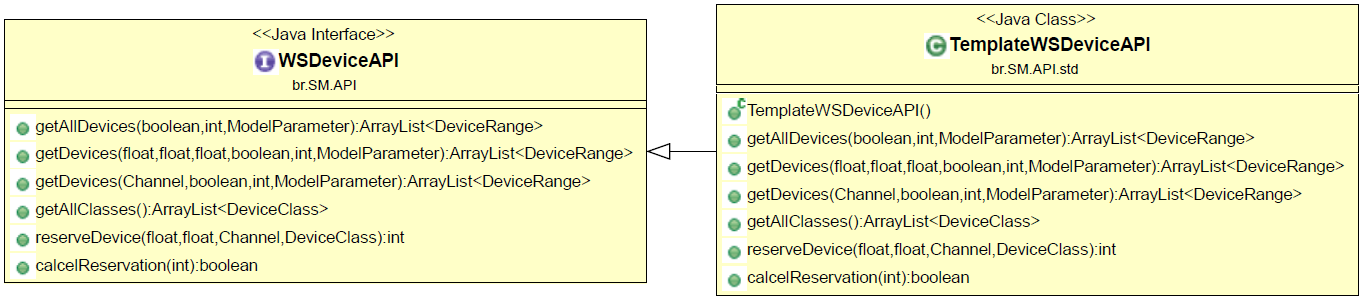
\includegraphics[width=1.0\textwidth]{figs/wsdeviceapi}
%\caption[\textit{Diagrama da classe \textit{WSDeviceAPI} }.]
%{Diagrama da classe \textit{WSDeviceAPI}.}
%\label{fig:WSDeviceAPI}
%\end{figure} 
%
%
%\FloatBarrier
%
%
%A classe \textit{WSDeviceAPI}, representada na figura~\ref{fig:WSDeviceAPI}, define seis métodos:
%
%\begin{lstlisting}
%
%	public ArrayList<DeviceRange> getAllDevices(boolean range, int modeltype, ModelParameter par);
%
%
%\end{lstlisting}
%
%
%Este método retorna uma lista com todos os dispositivos secundários presentes na base de dados, bem como o seu alcance.
%
%Ele é alcançado pela URL \textit{"http://servidor/SAM/devices/ws"}, utilizando o método GET. Pode ser utilizado, também a URL \textit{"http://servidor/SAM/ model/[modelo]/devices/ws"} onde \textit{[modelo]} indica o modelo de propagação que será utilizado para o cálculo dos alcances.
%
%Este método recebe alguns parâmetros, que são submetidos pelo cliente como parâmetros de URL:
%
%\begin{itemize}
%\item \textit{range} -- Um booleano que indica se a API deve calcular o alcance dos dispositivos ou não. É indicado pelo parâmetro de URL "range". Deve ser "true" ou "false". Se nenhum valor for indicado, será utilizado o valor padrão "false".
%\item \textit{modeltype} -- O modelo de propagação a ser utilizado. É indicado no corpo da URL. Só utilizado pela API de testes. A API padrão utiliza automaticamente o modelo Log Distance.
%\item \textit{par} -- Constituído de parâmetros específicos para um determinado modelo. Só utilizado pela API de testes. Cada modelo sabe quais parâmetros deve buscar. Para o modelo Log Distance o valor de \begin{math} \alpha \end{math} pode ser indicado pelo parâmetro de URL "alpha" .
%\end{itemize}
%
%Exemplo da URL utilizando a API padrão:
%
%\begin{lstlisting}	
%
%http://localhost:8182/SAM/devices/ws?
%	range=true
%
%\end{lstlisting}
%
%Exemplo da URL utilizando a API de teste:
%
%\begin{lstlisting}			
%
%http://localhost:8182/SAM/model/1/devices/ws?
%	range=true&alpha=2.5
%
%\end{lstlisting}
%
%
%A resposta desse método é uma lista de objetos \textit{DeviceRange}, como indicado na seção anterior.
%
%
%\begin{lstlisting}
%
%	public ArrayList<DeviceRange> getDevices(float lat, float lng, float ray, boolean range, 
%			int modeltype, ModelParameter par);
%
%\end{lstlisting}
%
%Este método retorna todos dispositivos secundários da base que estiverem dentro de um círculo, bem como o seu alcance. O centro e raio do círculo devem ser indicados pelo cliente.
%
%Ele é alcançado pela URL \textit{"http://servidor/SAM/devices/ws/location"}, utilizando o método GET. Pode ser utilizado, também a URL \textit{"http://servidor/SAM/ model/[modelo]/devices/ws/location"} onde \textit{[modelo]} indica o modelo de propagação que será utilizado para o cálculo dos alcances.
%
%Esse método recebe alguns parâmetros, que são submetidos pelo cliente como parâmetros de URL:
%
%\begin{itemize}
%\item \textit{range} -- Um booleano que indica se a API deve calcular o alcance dos dispositivos ou não. É indicado pelo parâmetro de URL "range". Deve ser "true" ou "false". Se nenhum valor for indicado, será utilizado o valor padrão "false".
%\item \textit{lat} -- A latitude do centro do círculo. É indicado pelo parâmetro de URL "lat".
%\item \textit{lng} -- A longitude do centro do círculo. É indicado pelo parâmetro de URL "lng".
%\item \textit{ray} -- O raio do círculo. É indicado pelo parâmetro de URL "ray". O valor de "ray" é em metros.
%\item \textit{modeltype} -- O modelo de propagação a ser utilizado. É indicado no corpo da URL. Só utilizado pela API de testes. A API padrão utiliza automaticamente o modelo Log Distance.
%\item \textit{par} -- Constituído de parâmetros específicos para um determinado modelo. Só utilizado pela API de testes. Cada modelo sabe quais parâmetros deve buscar. Para o modelo Log Distance o valor de \begin{math} \alpha \end{math} pode ser indicado pelo parâmetro de URL "alpha" .
%\end{itemize}
%
%
%Exemplo da URL utilizando a API padrão:
%
%\begin{lstlisting}	
%
%http://localhost:8182/SAM/devices/ws/location?
%	range=true&lat=-22.845882&lng=-43.08815&ray=1000
%
%\end{lstlisting}
%
%Exemplo da URL utilizando a API de teste:
%
%\begin{lstlisting}			
%
%http://localhost:8182/SAM/model/1/devices/ws/location?
%	range=true&lat=-22.845882&lng=-43.08815&ray=1000&alpha=2.5
%
%\end{lstlisting}
%
%
%A resposta desse método é uma lista de objetos \textit{DeviceRange}, como indicado na seção anterior.
%
%\begin{lstlisting}
%
%	public ArrayList<DeviceRange> getDevices(Channel cha, boolean range, int modeltype, ModelParameter par);
%
%\end{lstlisting}
%
%
%Este método retorna todos os dispositivos secundários que atuam em um determinado canal, bem como o seu alcance. O canal deve ser indicado pelo cliente.
%
%Ele é alcançado pela URL \textit{"http://servidor/SAM/devices/ws/channel"}, utilizando o método GET. Pode ser utilizado, também a URL \textit{"http://servidor/SAM/ model/[modelo]/devices/ws/channel"} onde \textit{[modelo]} indica o modelo de propagação que será utilizado para o cálculo dos alcances.
%
%Esse método recebe alguns parâmetros, que são submetidos pelo cliente como parâmetros de URL:
%
%\begin{itemize}
%\item \textit{cha} --  O canal a ser utilizado na busca. É indicado pelo parâmetro de URL "cha". Deve ser indicado o número do canal como definido pela ANATEL na tabela~\ref{table:tabcanal}.
%\item \textit{modeltype} -- O modelo de propagação a ser utilizado. É indicado no corpo da URL. Só utilizado pela API de testes. A API padrão utiliza automaticamente o modelo Log Distance.
%\item \textit{par} -- Constitui de parâmetros específicos para um determinado modelo. Só utilizado pela API de testes. Cada modelo sabe quais parâmetros deve buscar. Para o modelo Log Distance o valor de \begin{math} \alpha \end{math} pode ser indicado pelo parâmetro de URL "alpha" .
%\end{itemize}
%
%Exemplo da URL utilizando a API padrão:
%
%\begin{lstlisting}	
%
%http://localhost:8182/SAM/devices/ws/channel?
%	range=true&cha=4
%
%\end{lstlisting}
%
%Exemplo da URL utilizando a API de teste:
%
%\begin{lstlisting}			
%
%http://localhost:8182/SAM/model/1/devices/ws/channel?
%	range=true&cha=4&alpha=2.5
%
%\end{lstlisting}
%
%A resposta desse método é uma lista de objetos \textit{DeviceRange}, como indicado na seção anterior.
%
%
%\begin{lstlisting}
%
%	public ArrayList<DeviceClass> getAllClasses();
%
%\end{lstlisting}
%
%Esse método retorna todos os tipos de dispositivos secundários que a base de dados aceita. Ele deve ser usado pelo cliente para determinar em qual tipo ele se enquadra.
%
%Ele é alcançado pela URL \textit{"http://servidor/SAM/devices/ws/classes"}, utilizando o método GET.
%
%Exemplo da URL:
%
%\begin{lstlisting}	
%
%http://localhost:8182/SAM/devices/ws/classes
%
%\end{lstlisting}
%
%\FloatBarrier
%
%A resposta desse método é uma lista de objetos \textit{DeviceClass}, que tem as seguintes informações:
%
%\begin{itemize}
%\item Potência do dispositivo em Miliwatts -- \textit{DeviceClass.erp}
%\item Nome do dispositivo -- \textit{DeviceClass.name}
%\end{itemize}
%
%Exemplo de resposta em XML:
%
%\begin{lstlisting}	
%<list>
%  <br.SM.DO.DeviceClass>
%    <id>1</id>
%    <erp>10.0</erp>
%    <name>INTERNO BAIXO</name>
%  </br.SM.DO.DeviceClass>
%  <br.SM.DO.DeviceClass>
%    <id>2</id>
%    <erp>100.0</erp>
%    <name>EXTERNO</name>
%  </br.SM.DO.DeviceClass>
%  <br.SM.DO.DeviceClass>
%    <id>3</id>
%    <erp>50.0</erp>
%    <name>INTERNO ALTO</name>
%  </br.SM.DO.DeviceClass>
%</list>
%\end{lstlisting}
%
%
%
%\begin{lstlisting}
%
%	public int reserveDevice(float lat, float lng, Channel cha, DeviceClass cls);
%
%\end{lstlisting}
%
%Este método é utilizado pelo cliente para cadastrar um dispositivo secundário na base. Quando o cadastro é feito, a base reserva o canal indicado para o dispositivo. Devem ser informadas a localização do dispositivo, o canal que ele vai utilizar e o tipo de dispositivo.
%
%Ele é alcançado pela URL \textit{"http://servidor/SAM/devices/ws"}, utilizando o método PUT.
%
%Este método recebe alguns parâmetros, que são submetidos pelo cliente como parâmetros de URL:
%
%\begin{itemize}
%\item \textit{lat} -- A latitude do dispositivo. É indicado pelo parâmetro de URL "lat".
%\item \textit{lng} -- A longitude do dispositivo. É indicado pelo parâmetro de URL "lng".
%\item \textit{cha} -- O canal a ser utilizado na busca. É indicado pelo parâmetro de URL "cha". Deve ser indicado o número do canal como definido pela ANATEL na tabela~\ref{table:tabcanal}.
%\item \textit{cls} -- O tipo de dispositivo que deseja utilizar o WS. É indicado pelo parâmetro de URL "type".
%\end{itemize}
%
%
%Exemplo da URL:
%
%\begin{lstlisting}	
%
%http://localhost:8182/SAM/devices/ws?
%	lat=-22.845882&lng=-43.08815&cha=4&type=INTERNO+BAIXO
%
%\end{lstlisting}
%
%
%Este método retorna um inteiro para o cliente, que identifica o cadastro do dispositivo na base. Esse valor é utilizado para cancelar a reserva feita para o dispositivo. Se a resposta for 0, então a reserva não foi concluída
%
%\begin{lstlisting}
%
%	public boolean cancelReservation(int id);
%
%\end{lstlisting}
%
%
%
%Este método é responsável por cancelar uma reserva realizada por um dispositivo. O cliente deve indicar o dispositivo que foi cadastrado na base.
%
%Ele é alcançado pela URL \textit{"http://servidor/SAM/devices/ws"}, utilizando o método DELETE.
%
%Este método recebe um parâmetro, que é submetido pelo cliente como parâmetros de URL:
%\begin{itemize}
%\item \textit{id} -- A identificação da reserva a ser cancelada. É indicado pelo parâmetro de URL "id". Essa identificação é a resposta do método \textit{reserveDevice}
%\end{itemize}
%
%Exemplo da URL:
%
%\begin{lstlisting}	
%
%http://localhost:8182/SAM/devices/ws?
%	id=2
%
%\end{lstlisting}
%
%
%\subsubsection{TransmissionDeviceAPI}
%
%A classe \textit{TransmissionDeviceAPI}, representada na figura~\ref{fig:TransmissionDeviceAPI}, define 3 métodos:
%
%\begin{figure}[htb]
%\centering
%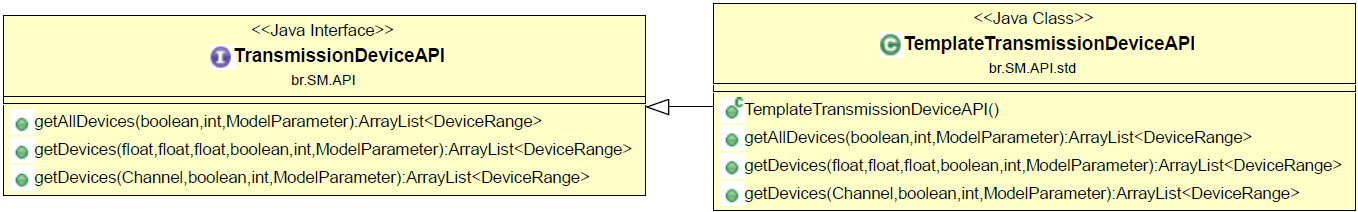
\includegraphics[width=1.0\textwidth]{figs/transdeviceapi}
%\caption[\textit{Diagrama da classe \textit{TransmissionDeviceAPI} }.]
%{Diagrama da classe \textit{TransmissionDeviceAPI}.}
%\label{fig:TransmissionDeviceAPI}
%\end{figure} 
%
%
%\begin{lstlisting}	
%
%public ArrayList<DeviceRange> getAllDevices(boolean range, int modeltype, 
%			ModelParameter par);
%
%\end{lstlisting}
%
%Este método retorna uma lista com todos os dispositivos de transmissão presentes na base de dados, bem como o seu alcance. Isso inclui todas as antenas e dispositivos secundários.
%
%Ele é alcançado pela URL \textit{"http://servidor/SAM/devices"}, utilizando o método GET. Pode ser utilizado, também a URL \textit{"http://servidor/SAM/model/[modelo]/ devices"} onde \textit{[modelo]} indica o modelo de propagação que será utilizado para o cálculo dos alcances.
%
%Este método recebe alguns parâmetros, que são submetidos pelo cliente como parâmetros de URL:
%
%\begin{itemize}
%\item \textit{range} -- Um booleano que indica se a API deve calcular o alcance dos dispositivos ou não. É indicado pelo parâmetro de URL "range". Deve ser "true" ou "false". Se nenhum valor for indicado, será utilizado o valor padrão "false".
%\item \textit{modeltype} -- O modelo de propagação a ser utilizado. É indicado no corpo da URL. Só utilizado pela API de testes. A API padrão utiliza automaticamente o modelo Log Distance.
%\item \textit{par} -- Constituído de parâmetros específicos para um determinado modelo. Só utilizado pela API de testes. Cada modelo sabe quais parâmetros deve buscar. Para o modelo Log Distance o valor de \begin{math} \alpha \end{math} pode ser indicado pelo parâmetro de URL "alpha" .
%\end{itemize}
%
%Exemplo da URL utilizando a API padrão:
%
%\begin{lstlisting}	
%
%http://localhost:8182/SAM/devices?
%	range=true
%
%\end{lstlisting}
%
%Exemplo da URL utilizando a API de teste:
%
%\begin{lstlisting}			
%
%http://localhost:8182/SAM/model/1/devices?
%	range=true&alpha=2.5
%
%\end{lstlisting}
%
%
%A resposta desse método é uma lista de objetos \textit{DeviceRange}, como indicado na seção anterior.
%
%
%\begin{lstlisting}	
%
%public ArrayList<DeviceRange> getDevices(float lat, float lng, float ray, boolean range, 
%			int modeltype, ModelParameter par);
%
%\end{lstlisting}
%
%
%Este método retorna todos os dispositivos de transmissão que estiverem dentro de um círculo, bem como o seu alcance. Isso inclui as antenas e dispositivos secundários. O centro e raio do círculo devem ser indicados pelo cliente.
%
%Ele é alcançado pela URL \textit{"http://servidor/SAM/devices/location"}, utilizando o método GET. Pode ser utilizado, também a URL \textit{"http://servidor/SAM/ model/[modelo]/devices/location"} onde \textit{[modelo]} indica o modelo de propagação que será utilizado para o cálculo dos alcances.
%
%Esse método recebe alguns parâmetros que são submetidos pelo cliente como parâmetros de URL:
%
%\begin{itemize}
%\item \textit{range} -- Um booleano que indica se a API deve calcular o alcance dos dispositivos ou não. É indicado pelo parâmetro de URL "range". Deve ser "true" ou "false". Se nenhum valor for indicado, será utilizado o valor padrão "false".
%\item \textit{lat} -- A latitude do centro do círculo. É indicado pelo parâmetro de URL "lat".
%\item \textit{lng} -- A longitude do centro do círculo. É indicado pelo parâmetro de URL "lng".
%\item \textit{ray} -- O raio do círculo. É indicado pelo parâmetro de URL "ray". O valor de "ray" é em metros.
%\item \textit{modeltype} -- O modelo de propagação a ser utilizado. É indicado no corpo da URL. Só utilizado pela API de testes. A API padrão utiliza automaticamente o modelo Log Distance.
%\item \textit{par} -- Constituído de parâmetros específicos para um determinado modelo. Só utilizado pela API de testes. Cada modelo sabe quais parâmetros deve buscar. Para o modelo Log Distance o valor de \begin{math} \alpha \end{math} pode ser indicado pelo parâmetro de URL "alpha" .
%\end{itemize}
%
%
%Exemplo da URL utilizando a API padrão:
%
%\begin{lstlisting}	
%
%http://localhost:8182/SAM/devices/location?
%	range=true&lat=-22.845882&lng=-43.08815&ray=1000
%
%\end{lstlisting}
%
%Exemplo da URL utilizando a API de teste:
%
%\begin{lstlisting}			
%
%http://localhost:8182/SAM/model/1/devices/location?
%	range=true&lat=-22.845882&lng=-43.08815&ray=1000&alpha=2.5
%
%\end{lstlisting}
%
%
%A resposta desse método é uma lista de objetos \textit{DeviceRange}, como indicado na seção anterior.
%
%
%\begin{lstlisting}	
%
%public ArrayList<DeviceRange> getDevices(Channel cha, boolean range, 
%			int modeltype, ModelParameter par);
%
%\end{lstlisting}
%
%Este método retorna todos os dispositivos de transmissão que atuam em um determinado canal, bem como o seu alcance. O canal deve ser indicado pelo cliente.
%
%Ele é alcançado pela URL \textit{"http://servidor/SAM/devices/channel"}, utilizando o método GET. Pode ser utilizado, também a URL \textit{"http://servidor/SAM/ model/[modelo]/devices/channel"} onde \textit{[modelo]} indica o modelo de propagação que será utilizado para o cálculo dos alcances.
%
%Esse método recebe alguns parâmetros, que são submetidos pelo cliente como parâmetros de URL:
%
%\begin{itemize}
%\item \textit{cha} --  O canal a ser utilizado na busca. É indicado pelo parâmetro de URL "cha". Deve ser indicado o número do canal como definido pela ANATEL na tabela~\ref{table:tabcanal}.
%\item \textit{modeltype} -- O modelo de propagação a ser utilizado. É indicado no corpo da URL. Só utilizado pela API de testes. A API padrão utiliza automaticamente o modelo Log Distance.
%\item \textit{par} -- Constitui de parâmetros específicos para um determinado modelo. Só utilizado pela API de testes. Cada modelo sabe quais parâmetros deve buscar. Para o modelo Log Distance o valor de \begin{math} \alpha \end{math} pode ser indicado pelo parâmetro de URL "alpha" .
%\end{itemize}
%
%Exemplo da URL utilizando a API padrão:
%
%\begin{lstlisting}	
%
%http://localhost:8182/SAM/devices/channel?
%	range=true&cha=4
%
%\end{lstlisting}
%
%Exemplo da URL utilizando a API de teste:
%
%\begin{lstlisting}			
%
%http://localhost:8182/SAM/model/1/devices/channel?
%	range=true&cha=4&alpha=2.5
%
%\end{lstlisting}
%
%A resposta desse método é uma lista de objetos \textit{DeviceRange}, como indicado na seção anterior.
